\section{Convergence of the out-forest}\label{sec.convoutforest}

Recall that $(\hat{F}_n(k),k\geq 1)$ is the sequence of out-forests given by the exploration, where we set $\hat{F}_n(k+1)=\hat{F}_n(k)$ if all in-half-edges have been paired at time $k$. In this section we will show that the \L ukasiewicz path and height process corresponding to $(\hat{F}_n(k),k\geq 1)$, denoted by $(\hat{S}^{+}_n(k),\hat{H}_n(k),k\geq 1)$, converge in distribution under rescaling. We show that this convergence occurs jointly with convergence in distribution under rescaling of $(\hat{S}^-_n(k),\hat{P}_n(k), k\geq 1)$, for $\hat{S}^-_n(k)$ the number of unpaired in-half-edges of vertices that have been discovered at time $k$, and $\hat{P}_n(k)$ the number of dummy leaves added in the first $k$ time-steps.  \\
We let $(B_t)_{t\geq 0}$ be a Brownian motion, and define
$$(\hat{B}_t,t\geq 0):=\left( B_t-\frac{\sigma_{-+}+\nu_-}{2\sigma_+ \mu}t^2, t\geq 0\right).$$ 
We define the reflected process $$(\hat{R}_t,t\geq 0)= \left(\hat{B}_t-\inf\left\{\hat{B}_s: s\leq t\right\},t\geq 0\right).$$

The main result of this section is as follows. 

\begin{theorem}\label{thm.convoutforest}
It holds that
\begin{align*}\left(n^{-1/3}\hat{S}^{+}_n\left(\lfloor n^{2/3}t\rfloor \right),n^{-1/3}\hat{H}_{n}\left(\lfloor n^{2/3}t\rfloor \right), t\geq 0\right)
\todist\left(\sigma_+ \hat{B}_t, \frac{2}{\sigma_+} \hat{R}_t, t\geq 0\right)\end{align*}
in $\D(\R_+,\R)^2$, and 
\begin{align*}\left( n^{-2/3}\hat{S}_n^-\left(\lfloor n^{2/3}t\rfloor \right), n^{-1/3}\hat{P}_n\left(\lfloor n^{2/3}t\rfloor \right), t\geq 0\right)\overset{p}{\to}\left(\nu_-t,  \frac{\nu_-}{2\mu} t^2, t\geq 0\right)\end{align*}
in $\D(\R_+,\R)^2$ as $n\to \infty$. 
\end{theorem}
We prove Theorem \ref{thm.convoutforest} by studying two other forests that are related to $\hat{F}_n(m_n)$ via a change of measure.  \\
The proof is structured as follows.
\begin{enumerate}
    \item \label{item.measurechangeexists} Let $(\mathbf{\hat{D}}_{n,1},\dots,\mathbf{\hat{D}}_{n,R_n})$ denote the in- and out-degree pairs in order of discovery. Let $\mathbf{Z}_1, \mathbf{Z}_2, \ldots$ be an i.i.d. sequence of $\N\times \N$-valued random variables, $\mathbf{Z}_i:=(Z_i^-,Z_i^+)$, such that 
    $$\P(Z_i^-=k^-, Z_i^+=k^+)=\frac{k^-\P(D^-=k^-,D^+=k^+)}{\mu}.$$
    Then, we show that the law of $(\mathbf{\hat{D}}_{n,1},\dots,\mathbf{\hat{D}}_{n,m})$ conditional on $\sum_{i=1}^n D_i^-=\sum_{i=1}^n D_i^+$ and $m \leq R_n$ is absolutely continuous with respect to that of $(\mathbf{Z}_1,\dots, \mathbf{Z}_m)$, and we show the convergence of the Radon-Nikodym derivative $\phi_m^n$ for $m=O(n^{2/3})$. This is the content of Subsection \ref{subsec.measurechange}.
    \item Let $(\mathbf{Z}_i,i\geq 1)$ be a sequence of i.i.d.\ copies of $\mathbf{Z}$. Point \ref{item.measurechangeexists} motivates us to study a Bienaymé forest with offspring distributed as $Z_1^+$. Call this forest $(F(k),k\geq 1)$. The convergence of the \L ukasiewicz path of $(F(k),k\geq 1)$ under rescaling follows from Donsker's theorem.
    \item In Subsection \ref{subsec.purpleleavesGWforest}, we modify $(F(k),k\geq 1)$ in order to include dummy leaves. We add extra randomness, approximating the procedure described in Lemma \ref{lemma.sampleoutforest}, in such a way that at some time-steps, a dummy leaf is added. We call the resulting forest $(F^p_n(k),k\geq 1)$. We respect the order of the degrees in $(F(k),k\geq 1)$, in the sense that for any $k$, the $k^{th}$ black vertex in $(F^p_n(k),k\geq 1)$ has the same number of children as the $k^{th}$ vertex in $(F(k),k\geq 1)$. $(F^p_n(k),k\geq 1)$ depends on $n$, because the probability of finding a dummy leaf depends on $n$. We then show that the \L ukasiewicz path and height process corresponding to $(F^p_n(k),k\geq 1)$ converge under rescaling, jointly with the convergence of the \L ukasiewicz path and height process corresponding to $(F(k),k\geq 1)$ under rescaling up to time $O(n^{2/3})$.
    \item We show convergence under rescaling of $(\hat{F}_n(k),k\geq 1)$ up to time $O(n^{2/3})$ by applying the measure change to $(F^p_n(k),k\geq 1)$ and showing that the resulting process is a good approximation of $(\hat{F}_n(k),k\geq 1)$. 
\end{enumerate}

\subsection{The measure change and its convergence}\label{subsec.measurechange}

The following theorem asserts existence of the measure change and gives the scaling limit of the measure change, jointly with the random walks $Y^-$ and $Y^+$. The measure change is under the conditioning $m \leq R_n$ which is an event that occurs with high probability when $m = \Theta(n^{2/3})$. (Indeed, $R_n$ is equal to the number of vertices with in-degree unequal to $0$, so $R_n\overset{d}{=}\mathrm{Binom}(n,\P(D^-\neq 0))$, which is $O(n)$ with high probability.)

\section{Analysis of the measure change}
\label{sec:measure-change}

Recall $(\hat{\vD}_{n, 1}, \hat{\vD}_{n, 2}, \ldots, \hat{\vD}_{n, n})$ are are the degree pairs of the vertices in order of discovery, and that $R_n$ is the number of vertices with positive in-degree. The behaviour of the $\hat{\vD}_{m, n}$ for $m \leq R_n$ and $m > R_n$ is rather different. Before $R_n$, new vertices are discovered with probability proportional to their in-degree. After $R_n$, all vertices with positive in-degree have already been discovered and we choose to explore the remaining vertices in some uniform order.

Later in \cref{sec.convSCCs}, we show that we only need to consider timescales of the order of $m = \Theta(n^{2/3})$. Let $p = \P(D^- > 0)$ such that $R_n$ is distributed as a $\text{Binomial}(n, p)$ random variable. We show now that the probability that $m \leq R_n$ will converge exponentially to 1.
\begin{lemma}
    If $m = \Theta(n^{2/3})$ then there exists $c > 0$ such that $\P(R_n < m) < e^{-c n}$.
\end{lemma}
\begin{proof}
    If $m = \Theta(n^{2/3})$ then $\E[R_n] - m = pn - m = \Theta(n)$. Thus by Hoeffding's inequality
    \begin{equation*}
        \P(R_n < m)
        = \P\left(\E[R_n] - R_n > \E[R_n] - m\right)
        \leq e^{-\frac{2}{n} (\E[R_n] - m)^2} < e^{-cn}
    \end{equation*}
    for some $c > 0$.
\end{proof}
Hence it is sensible to prove results on the event that $m \leq R_n$.

When discussing the criticality condition, we gave heuristics showing that the limiting distribution of $\hat{D}_{n, 1}$ is given by $\vZ$ where
\begin{equation*}
    \P(Z^- = k^-, Z^+ = k^+) = \frac{k^-}{\mu}\P(D^- = k^-, D^+ = k^+).
\end{equation*}
Similarly, $\hat{D}_{n, 2}$ is also approximately distributed like $\vZ$ for large $n$, and so on. In this section we in fact prove a precise relation between $\hat{\vD}_{n, 1}, \ldots, \hat{\vD}_{n, m}$ and the sequence $\vZ_1, \vZ_2, \ldots$ of i.i.d.\ copies of $\vZ$.

The results proved in this section do not actually require the criticality condition, so let us define notation for the mean of the $Z_i^{\pm}$ and the two corresponding centered random walks. Let
\begin{equation*}
    \lambda_{\pm} = \E[Z^{\pm}_1]
    \quad \text{and} \quad
    V^{\pm}(n) = \textstyle \sum_{i=1}^n (Z^{\pm}_i - \lambda_{\pm}).
\end{equation*}
The criticality condition is then equivalent to assuming $\lambda_+ = 1$. We also define the notation
\begin{equation*}
    \Xi^{\pm}_{n-m} = \sum_{i=m+1}^n D_i^{\pm}
    \quad \text{and} \quad
    \Delta_n = \Xi^-_n - \Xi^+_n
\end{equation*}
such that $\{\Delta_n = 0\}$ is the event that the total out-degree is equal to the total in-degree.

The following lemma asserts the existence of the measure change $\phi^n_m$, and its joint scaling limit with the random walks $V^-$ and $V^+$ when $m = \floor{n^{2/3} T}$ for some $T > 0$.
\begin{proposition}
    \label{prop:measure-change-no-crit}
    For all positive integers $n$ and $m$ such that $m \leq n$, there exists a function $\phi^n_m: (\N \times \N)^n \to [0, \infty)$ such that 
    \begin{equation*}
        \E\left[\left.u(\hat{\vD}_{n, 1}, \ldots, \hat{\vD}_{n, m}) \one\{R_n \geq m\} \right| \Delta_n = 0\right]
        = \E[u(\vZ_1, \ldots, \vZ_m) \phi^n_m(\vZ_1, \ldots, \vZ_m)]
    \end{equation*}
    for all bounded test functions $u: (\N \times \N)^m \to \R$. Define
    \begin{equation*}
        \Phi(n, m) = \phi^n_m(\vZ_1, \ldots, \vZ_m).
    \end{equation*}
    Further, let $(W^-, W^+)$ be a pair of correlated standard Brownian motions with correlation $\corr(Z_1^-, Z_1^+)$ and, for $T > 0$, define
    \begin{equation*}
        \Phi(T) = \exp\left( 
            - \frac{\sigma_-}{\mu} \int_0^T s \dif W_s^- 
            - \frac{\sigma_-^2}{6 \mu^2} T^3
        \right).
    \end{equation*}
    Then for all $T > 0$,
    \begin{align*}
        &\left( 
            \Phi(n, \floor{n^{2/3} T}),
            \left(
                n^{-1/3} V^-\left( \floor{n^{2/3} t} \right),
                n^{-1/3} V^+\left( \floor{n^{2/3} t} \right)
            \right)_{t \in [0, T]}
        \right) \\
        & \hspace{23em} \todist \left( 
            \Phi(T),
            (\sigma_- W^-_t, \sigma_+ W^+_t)_{t \in [0, T]}
        \right)
    \end{align*}
    in $\R \times \D([0, T], \R^2)$ as $n \to \infty$, even in the absence of the criticality condition.
\end{proposition}
The rest of this section is dedicated to proving this proposition.

\subsection{Exact form of the measure change}

To determine the exact form of the measure change, we first need to know the law of the ordering of the first $R_n$ vertices. Let $\cI_n = \{i \in [n] : D_i^- > 0\}$. The first $R_n$ vertices we explore in \cref{alg:edfs} will have positive in-degree, thus there exists a random bijection $\Sigma_n: [R_n] \to \cI_n$ such that $\hat{\vD}_{n, i} = \vD_{\Sigma_n(i)}$ for $i = 1, \ldots, R_n$. 
\begin{lemma}
    $\Sigma_n$ has law
    \begin{equation*}
        \P(\Sigma_n = \sigma \mid \vD_1, \ldots, \vD_n)
        = \prod_{i=1}^{R_n} \frac{D^-_{\sigma(i)}}{\sum_{j=i}^{R_n} D^-_{\sigma(j)}}.
    \end{equation*}
    for all bijections $\sigma: [R_n] \to \cI_n$.
\end{lemma}
\begin{proof}
    In \cref{alg:edfs}, a vertex first becomes explored in two ways. Either it is at the start of an out-component or it is discovered when an out-half-edge is paired to one its in-half-edges.

    Suppose we have explored $m$ vertices and $m < R_n$. If the next vertex is explored by pairing one of its in-half-edges, then we have chosen it with probability proportional to its in-degree since in- and out-half-edges are paired uniformly at random. Otherwise, it is at the start of a new out-component, and since $m < R_n$, there are still vertices of positive in-degree. Thus we still pick a new vertex with probability proportional to its in-degree.

    Therefore in all cases,
    \begin{align*}
        &\P(\Sigma_n(m+1) = \sigma(m+1) \mid \Sigma_n(1) = \sigma(1), \ldots, \Sigma_n(m) = \sigma(m), \vD_1, \ldots, \vD_n) \\
        =&  \frac{D^-_{\sigma(m+1)}}{\sum_{i \in \cI_n} D_i^- - \sum_{j=1}^m D^-_{\sigma(j)}}
        = \frac{D^-_{\sigma(m+1)}}{\sum_{j=m+1}^{R_n} D^-_{\sigma(j)}}.
    \end{align*} 
    From this, repeated applications of the definition of conditional probability yields the desired result.
\end{proof}

Next we establish the form of the measure change when we condition on the exact value of $R_n$ but not $\Delta_n = 0$.

\begin{lemma}
    \label{lem:exact-measure-change-no-conditioning}
    For all integers $0 \leq r \leq n$ and test functions $u: (\N \times \N)^r \times \N \to \R$,
    \begin{equation*}
        \E \left[ u\left( 
            \hat{\vD}_{n, 1}, \ldots, \hat{\vD}_{n, r}, \textstyle \sum_{i \in \cI_n^c} D_i^+
        \right) \,\middle\vert\, R_n = r \right] \\
        =
        \E \left[
            u\left( \vZ_1, \ldots, \vZ_r, \textstyle \sum_{i = 1}^{n-r} E_i^+ \right)
            \psi_r(\vZ_1, \ldots, \vZ_r)
        \right]
    \end{equation*}
    where
    \begin{equation*}
        \psi_r(\vk_1, \ldots, \vk_r) =
        \frac{1}{p^r} \prod_{i=1}^r \frac{(r - i + 1)\mu}{\sum_{j=i}^r k_i^-}.
    \end{equation*}
    and $E_1^+, E_2^+, \ldots$ are i.i.d.\ random variables such that $E_i^+$ has the same distribution as $D^+$ conditioned on $D^- = 0$. We take the sequences $(E_i^+)_{i \geq 1}$ and $(\vZ_i)_{i \geq 1}$ to be independent.
\end{lemma}

\begin{proof}
    For any $\vk_1, \ldots, \vk_m \in \N^+ \times \N$ for all $i$ and $s \in \N$.
    \begin{align*}
        & \P\left(\hat{\vD}_{n, 1} = \vk_1, \ldots, \hat{\vD}_{n, r} = \vk_r, \textstyle \sum_{i \in \cI_n^c} D_i^+ = s, R_n = r \right) \\
        =& \sum_{\substack{I \subset [n] \\ \abs{I} = r}} \sum_{\sigma: [r] \to I}
        \P\left(\vD_{\Sigma_n(1)} = \vk_1, \ldots, \vD_{\Sigma_n(r)} = \vk_r, \textstyle \sum_{i \in \cI_n^c} D_i^+ = s, \cI_n = I, \Sigma_n = \sigma \right)
    \end{align*}
    where the second summation is taken over all bijections $\sigma: [r] \to I$. We examine a single summand.
    \begin{align*}
        &\P\left(\vD_{\Sigma_n(1)} = \vk_1, \ldots, \vD_{\Sigma_n(r)} = \vk_r, \textstyle \sum_{i \in \cI_n^c} D_i^+ = s, \cI_n = I, \Sigma_n = \sigma \right) \\
        =&\P\left(
            \vD_{\sigma(j)} = \vk_j\ \text{for $j = 1, \ldots, r$},
            \textstyle \sum_{i \in I^c} D_i^+ = s,
            D^-_i = 0\ \text{for $i \in I^c$},
            \Sigma_n = \sigma
            \right)  \\
        =& \prod_{i=1}^r \frac{k_i^-}{\sum_{j=i}^r k_j^-}
        \times \prod_{i=1}^r \lambda_{\vk_i}
        \times \P\left( 
            \textstyle \sum_{i \in I^c} D_i^+ = s,
            D^-_i = 0\ \text{for $i \in I^c$}
         \right).
    \end{align*}
    where $\lambda_{\vk} = \P(\vD_1 = \vk)$. We have
    \begin{equation*}
        \P\left( 
            \textstyle \sum_{i \in I^c} D_i^+ = s,
            D^-_i = 0\ \text{for $i \in I^c$}
         \right)
         = (1-p)^{n-r} \P\left( 
             \textstyle \sum_{i=1}^{n-r} E^+_i = s
          \right).
    \end{equation*}
    Also
    \begin{align*}
        \prod_{i=1}^r \frac{k_i^-}{\sum_{j=i}^r k_j^-} \times \prod_{i=1}^r \lambda_{\vk_i}
        &= \prod_{i=1}^r \frac{k_i^-}{\mu} \lambda_{\vk_i} \times \prod_{i=1}^r \frac{\mu}{\sum_{j=i}^r k_j^-} \\
        &= \P(\vZ_1 = \vk_1, \ldots, \vZ_r = \vk_r)
        \times \prod_{i=1}^r \frac{\mu}{\sum_{j=i}^r k_j^-}.
    \end{align*}
    Therefore
    \begin{align*}
        & \P\left(\hat{\vD}_{n, 1} = \vk_1, \ldots, \hat{\vD}_{n, r} = \vk_r, \textstyle \sum_{i \in \cI_n^c} D_i^+ = s, R_n = r \right) \\
        =& \binom{n}{r} \times r!
        \times \prod_{i=1}^r \frac{\mu}{\sum_{j=i}^r k_j^-} \times (1-p)^{n-r}
        \times \P\left(\vZ_1 = \vk_1, \ldots, \vZ_r = \vk_r, \textstyle \sum_{i=1}^{n-r} E_i^+ = s \right) \\
        =& \binom{n}{r} p^r (1-p)^{n-r} \times \frac{1}{p^r} \prod_{i=1}^r \frac{(r-i+1) \mu}{\sum_{j=i}^r k_i^-}
        \times \P\left(\vZ_1 = \vk_1, \ldots, \vZ_r = \vk_r, \textstyle \sum_{i=1}^{n-r} E_i^+ = s \right).
    \end{align*}
    Finally dividing by $\P(R_n = r) = \binom{n}{r} p^r (1-p)^{n-r}$ gives the desired measure change.
\end{proof}

Using the previous lemma we can prove existence and give the exact form of the desired measure change $\phi^n_m$.

\begin{lemma}
    \label{lem:exact-measure-change}
    For all $m \leq n$ and test functions $u: (\N \times \N)^m \to \R$,
    \begin{equation*}
        \E \left[
            u\left( \hat{\vD}_{n, 1}, \ldots, \hat{\vD}_{n, m} \right)
            \one\{R_n \geq m\}
            \,\middle\vert\,
            \Delta_n = 0
        \right] \\
        =
        \E \left[
            u\left( \vZ_1, \ldots, \vZ_m \right)
            \phi^n_m(\vZ_1, \ldots, \vZ_m)
        \right],
    \end{equation*}
    where
    \begin{align*}
        \phi^n_m(\vk_1, \ldots, \vk_m) =
        \frac{1}{\P(\Delta_n = 0)} \E\left[ 
            \one \left\{ \Delta_{n-m} = \sum_{i=1}^m (k_i^+ - k_i^-) \right\}
            \prod_{i=1}^m \frac{(n - i + 1) \mu}{\sum_{j=1}^m k_j^- + \Xi_{n-m}^-}
        \right].
    \end{align*}
\end{lemma}

\begin{proof}
    By \cref{lem:exact-measure-change-no-conditioning}, for all $r \geq m$
    \begin{align*}
        &\E \left[ 
            u\left( 
                \hat{\vD}_{n, 1}, \ldots, \hat{\vD}_{n, m}
             \right)
            \one\{\Delta_n = 0\}
            \, \middle\vert \,
            R_n = r
         \right] \\
        =&\E \left[ 
            u\left( \vZ_1, \ldots, \vZ_m \right)
            \one \left\{ 
                \sum_{i=1}^r (Z_i^- - Z_i^+) - \sum_{i=1}^{n-r} E_i^+ = 0
             \right\}
             \frac{1}{p^r} \prod_{i=1}^r \frac{(r - i + 1) \mu}{\sum_{j=i}^r Z_j^-}
         \right] \\
        =&\E \left[ 
            u\left( \vZ_1, \ldots, \vZ_m \right)
            \E \left[ 
                \one \left\{ 
                    \sum_{i=1}^r (Z_i^- - Z_i^+) - \sum_{i=1}^{n-r} E_i^+ = 0
                \right\}
                \frac{1}{p^r} \prod_{i=1}^r \frac{(r - i + 1) \mu}{\sum_{j=i}^r Z_j^-}
                \, \middle \lvert \,
                \vZ_1, \ldots, \vZ_m
             \right]
         \right] \\
        =&\E \left[ 
            u\left( \vZ_1, \ldots, \vZ_m \right)
            \tilde{\gamma}^{n, m}_r (\vZ_1, \ldots, \vZ_m)
         \right],
    \end{align*}
    where
    \begin{align*}
        \tilde{\gamma}^{n, m}_r (\vk_1, \ldots, \vk_m)
        &= \E \Bigg[ 
            \one \left\{ 
                \sum_{i=m+1}^r (Z_i^- - Z_i^+) - \sum_{i=1}^{n-r} E_i^+ = \sum_{i=1}^m (k_i^+ - k_i^-)
            \right\} \times \\
            &\hspace{5em}
            \frac{1}{p^m} \prod_{i=1}^m \frac{(r - i + 1) \mu}{\sum_{j=i}^m k_j^- + \sum_{j=m+1}^r Z_j^-}
            \frac{1}{p^{r-m}} \prod_{i=m+1}^r \frac{(r - i + 1) \mu}{\sum_{j=i}^r Z_j^-}
        \Bigg] \\
        &= \E \Bigg[ 
            \one \left\{ 
                \sum_{i=1}^{r-m} (Z_i^- - Z_i^+) - \sum_{i=1}^{n-r} E_i^+ = \sum_{i=1}^m (k_i^+ - k_i^-)
            \right\} \times \\
            &\hspace{5em}
            \frac{1}{p^m} \prod_{i=1}^m \frac{(r - i + 1) \mu}{\sum_{j=i}^m k_j^- + \sum_{j=1}^{r-m} Z_j^-}
            \frac{1}{p^{r-m}} \prod_{i=1}^{r-m} \frac{(r - m - i + 1) \mu}{\sum_{j=i}^{r-m} Z_j^-}
        \Bigg],
    \end{align*}
    since $(\vZ_i)_{i=m+1}^r$ has the same law as $(\vZ_i)_{i=1}^{r-m}$. Then applying \cref{lem:exact-measure-change-no-conditioning} again shows that
    \begin{align*}
        \tilde{\gamma}^{n, m}_r (\vk_1, \ldots, \vk_m)
        &= \E \Bigg[ 
            \one \left\{ 
                \sum_{i=1}^{r-m} (\hat{D}_{n-m,i}^- - \hat{D}_{n-m,i}^+) - \sum_{i \in \cI_{n-m}^c} D_i^+ = \sum_{i=1}^m (k_i^+ - k_i^-)
            \right\} \times \\
            &\hspace{8em}
            \frac{1}{p^m} \prod_{i=1}^m \frac{(r - i + 1) \mu}{\sum_{j=i}^m k_j^- + \sum_{j=1}^{r-m} \hat{D}_{n-m,j}^-}
            \Biggm|
            R_{n-m} = r-m
        \Bigg].
    \end{align*}
    Conditional on $R_{n-m} = r-m$, we have
    \begin{equation*}
        \sum_{j=1}^{r-m} (\hat{D}_{n-m,j}^- - \hat{D}_{n-m,j}^+) - \sum_{i \in \cI_{n-m}^c} D_i^+ = \Delta_{n-m}
        \quad \text{and} \quad
        \sum_{j=1}^{r-m} \hat{D}_{n-m, j}^- = \Xi^-_{n-m}.
    \end{equation*}
    Therefore,
    \begin{align*}
        \tilde{\gamma}^{n, m}_r (\vk_1, \ldots, \vk_m)
        &= \E \left[
            \frac{1}{p^m} \prod_{i=1}^m \frac{(r - i + 1) \mu}{\sum_{j=i}^m k_j^- + \Xi_{n-m}^-} \one_{A_n}
            \, \middle \vert \,
            R_{n-m} = r-m
        \right],
    \end{align*}
    where
    \begin{equation*}
        A_n(\vk_1, \ldots, \vk_m) = \left\{ \Delta_{n-m} =  \sum_{i=1}^m (k_i^+ - k_i^-) \right\}.
    \end{equation*}
    Hence,
    \begin{align*}
        \E \left[ 
            u\left( 
                \hat{\vD}_{n, 1}, \ldots, \hat{\vD}_{n, m}
             \right)
            \one\{R_n \geq m, \Delta_n = 0\}
         \right]
        =\E \left[ 
            u\left( \vZ_1, \ldots, \vZ_m \right)
            \tilde{\phi}^n_m(\vZ_1, \ldots, \vZ_m)
         \right],
    \end{align*}
    where
    \begin{align*}
        &\tilde{\phi}^n_m(\vk_1, \ldots, \vk_m) \\
        =& \sum_{r=m}^n \binom{n}{r} p^r (1-p)^{n-r} 
        \E \left[
            \frac{1}{p^m} \prod_{i=1}^m \frac{(r - i + 1) \mu}{\sum_{j=i}^m k_j^- + \Xi_{n-m}^-} \one_{A_n}
            \, \middle \vert \,
            R_{n-m} = r-m
        \right] \\
        =& \sum_{l=0}^{n-m} \binom{n}{l+m} p^{l+m} (1-p)^{n-m-l} 
        \E \left[
            \frac{1}{p^m} \prod_{i=1}^m \frac{(l + m - i + 1) \mu}{\sum_{j=i}^m k_j^- + \Xi_{n-m}^-} \one_{A_n}
            \, \middle \vert \,
            R_{n-m} = l
        \right].
    \end{align*}
    We wish to view the sum as an expectation over $R_{n-m}$. In order to do this, we rewrite the expression so that we are taking a sum over the probabilities of a $\text{Binomial}(n-m, p)$ distribution. We can calculate
    \begin{equation*}
        \frac{\binom{n}{l+m} p^{l+m} (1-p)^{n-m-l}}{\binom{n-m}{l} p^l (1-p)^{n-m-l}}
        = p^m \prod_{i=1}^m \frac{(n-i+1)}{(l+m-i+1)}.
    \end{equation*}
    Therefore,
    \begin{align*}
        \tilde{\phi}^n_m(\vk_1, \ldots, \vk_m)
        &= \sum_{l=1}^{n-m} \binom{n-m}{l} p^l (1-p)^{n-m-l}
        \E \left[
            \prod_{i=1}^m \frac{(n - i + 1) \mu}{\sum_{j=i}^m k_j^- + \Xi_{n-m}^-} \one_{A_n}
            \, \middle \vert \,
            R_{n-m} = l
        \right] \\
        &= \E\left[ 
            \E \left[
                \prod_{i=1}^m \frac{(n - i + 1) \mu}{\sum_{j=i}^m k_j^- + \Xi_{n-m}^-} \one_{A_n}
                \, \middle \vert \,
                R_{n-m}
            \right]
         \right] \\
         &= \E \left[
            \prod_{i=1}^m \frac{(n - i + 1) \mu}{\sum_{j=i}^m k_j^- + \Xi_{n-m}^-} \one_{A_n}
        \right].
    \end{align*}
    Finally, dividing by $\P(\Delta_n = 0)$ yields the desired form of $\phi^n_m$.
\end{proof}

\subsection{Asymptotic lower bound on the measure change}

Recall that our goal in \cref{prop:measure-change-no-crit} is to determine the limiting distribution of
\begin{equation*}
    \Phi(n, m) = \phi^n_m(\vZ_1, \ldots, \vZ_m),
\end{equation*}
as $n \to \infty$, in the regime where $m = \Theta(n^{2/3})$. When dealing with convergence in distribution, it is suffcient and necessary to work on a sequence of events occuring with high probability. In particular, for the proof of \cref{prop:measure-change-no-crit}, we work on the event $\walkDeviationEvent_m$ where
\begin{align*}
    \walkDeviationEvent_m
    &= \Bigg\{ 
    \max_{i=1, \ldots, m } \abs*{
        \textstyle\sum_{j=1}^i (Z^{-}_j - \lambda_{-}) 
    } \leq m^{1/2} \log(m) \\
    &\hspace{13em} \text{and} \quad
    \max_{i=1, \ldots, m } \abs*{
        \textstyle\sum_{j=1}^i (Z^{+}_j - \lambda_{+}) 
    } \leq m^{1/2} \log(m)
    \Bigg\}.
\end{align*}
This says that the centered random walks corresponding to $Z^+_i$ and $Z^-_i$ both do not deviate by more than $m^{1/2} \log(m)$ in the first $m$ steps. The conditions in \cref{subsec:model-description} ensure each $Z^+_i$ and $Z^-_i$ has finite variance, thus this event will occur with high probability. 

The following lemma is an analogue of \citet[Lemma 6.7]{conchon--kerjanStableGraphMetric2020}. In it we prove a deterministic lower bound on $\phi^n_m(\vk_1, \ldots, \vk_m)$, for all $\vk_1, \ldots, \vk_m$ corresponding to the event $\walkDeviationEvent_m$, up to an error which vanishes as $n \to \infty$.
\begin{proposition}
    \label{prop:measure-change-approx}
    Define
    \begin{equation*}
        s^{\pm}(i) = \textstyle{\sum_{j=1}^i (k_i^{\pm} - \lambda_{\pm})}.
    \end{equation*}
    Suppose that $\vk_1, \ldots, \vk_m$ are such that
    \begin{equation}
        \label{eq:s-condition}
        \max_{i=1, \ldots, m} \abs{s^{-}(i)} \leq m^{\frac{1}{2}} \log(m)
        \quad \text{and} \quad
        \max_{i=1, \ldots, m} \abs{s^{+}(i)} \leq m^{\frac{1}{2}} \log(m)
    \end{equation}
    Then in the regime $m = \Theta(n^{2/3})$, as $n \to \infty$,
    \begin{equation*}
        \phi^n_m(\vk_1, \ldots, \vk_m)
        \geq \exp\left( \frac{1}{\mu n} \sum_{i=0}^m (s^-(i) - s^-(m)) - \frac{\sigma_-}{6 \mu^2} \frac{m^3}{n^2} \right) + \littleo(1),
    \end{equation*}
    where the $\littleo(1)$ error term is independent of $\vk_1, \ldots, \vk_m$ satisfying the assumption in \cref{eq:s-condition}.
\end{proposition}


The fact that we only prove a lower bound may seem strange at first. To understand why this is sufficient, first note that all measure changes are non-negative random variables and have expectation 1. Hence if the sequence of lower bounds on the measure changes converge to a limit that also has expectation 1, then we have not have lost a significant amount of probability mass. It follows that the measure changes converge to the same limit as the lower bounds. This is made formal by \citet[Lemma 4.8]{conchon--kerjanStableGraphMetric2020}. In \cref{prop:measure-change-no-crit} we are considering the joint convergence of the measure change with two other random walks, and thus we adapt \cite[Lemma 4.8]{conchon--kerjanStableGraphMetric2020} to allow for an additional coordinate that is converging jointly with the first coordinate.
\begin{lemma}
    \label{lem:sandwiching-lemma}
    Let $(X_n, Y_n, Z_n)_{n \geq 1}$ be a sequence of $[0, \infty) \times [0, \infty) \times S$-valued random variables where $S$ is a metric space. Suppose there exists a $[0, \infty) \times S$-valued random variable $(Y, Z)$ such that the following holds:
    \begin{enumerate}
        \item $(Y_n, Z_n) \todist (Y, Z)$ as $n \to \infty$.
        \item $X_n \geq Y_n$ almost surely for all $n$.
        \item $\E[X_n] = 1$ for all $n$ and $\E[Y] = 1$.
    \end{enumerate}
    Then $(X_n, Z_n) \todist (Y, Z)$ also. Moreover $(X_n)_{n \geq 1}$ is a sequence of uniformly integrable random variables.
\end{lemma}
The proof of this lemma is obtained by simply adding the corresponding $Z_n$ or $Z$ coordinate to quantities in the proof of \cite[Lemma 4.8]{conchon--kerjanStableGraphMetric2020} and so we will not repeat it here.

\subsubsection{Discrete local limit theorem}

To prove \cref{prop:measure-change-approx}, we first need to understand the denominator of $\phi^n_m$, which, as given by \cref{lem:exact-measure-change}, is $\P(\Delta_n = 0)$. The random variable $\Delta_n$ is a sum of independent integer-valued random variables and the asymptotic behaviour of such a sum being equal to some value is described by the discrete local limit theorem. Such a theorem was first proven by \citet{gnedenkoLocalLimitTheorem1948}. Here we borrow the presentation from \citet[Section 3.5]{durrettProbabilityTheoryExamples2019}.

Let $X_1, X_2, \ldots$ be i.i.d.\ integer-valued random variables with mean $\mu$ and finite variance $\sigma^2$. Then, by the central limit theorem,
\begin{equation*}
    \frac{ \sum_{i=1}^n X_i - n \mu }{\sigma \sqrt{n}}
    \todist
    N(0, 1)
\end{equation*}
as $n \to \infty$. Thus we expect $\sum_{i=1}^n X_i$ to be distributed like a $N(n \mu, n \sigma^2)$ random variable for large values of $n$. Therefore the probability mass function of $\sum_{i=1}^n X_i$ should be well approximated by the probability density function of a $N(n \mu, n \sigma^2)$ distribution, i.e.
\begin{equation*}
    \P\big( \textstyle \sum_{i=1}^n X_i = s \big)
    \approx
    \frac{1}{\sqrt{2 \pi n \sigma^2}}  \exp \left(
        \frac{-(s - n \mu)^2}{2 n \sigma^2}
    \right)
\end{equation*}
for all integers $s$. Specifically we hope that
\begin{equation}
    \label{eq:llt-approx}
    \sup_{s \in \Z} \abs*{
        \P\big( \textstyle \sum_{i=1}^n X_i = s \big) 
        -
        \frac{1}{\sqrt{2 \pi n \sigma^2}}  \exp \left(
            \frac{-(s - n \mu)^2}{2 n \sigma^2}
        \right)
    } = \littleo(n^{-1/2}).
\end{equation}

This, however, is not always the case. Suppose, for example, that each $X_i$ is almost surely even such that $\P\left( \sum_{i=1}^n X_i = s \right) = 0$ for all odd $s$. Let $s_n$ be the closest odd integer to $n \mu$. Then
\begin{equation*}
    \sup_{s \in \Z} \abs*{
        \P\big( \textstyle \sum_{i=1}^n X_i = s \big) 
        -
        \frac{1}{\sqrt{2 \pi n \sigma^2}}  \exp \left(
            \frac{-(s - n \mu)^2}{2 n \sigma^2}
        \right)
    }
    \geq
    \frac{1}{\sqrt{2 \pi n \sigma^2}}  \exp \left(
        \frac{-(s_n - n \mu)^2}{2 n \sigma^2}
    \right)
    = 
    \Theta(n^{ -1/2 }).
\end{equation*}

Fortunately this kind of periodic behaviour can be mitigated by normalizing the random variables. A one-dimensional random variable $X$ is \emph{lattice} if it is not almost surely constant, and there exists $h > 0$ and $c \in \R$ such that $X \in c + h\Z$ almost surely. The largest such $h$ is called the \emph{span} of $X$. For example, if $X$ is almost surely even then $X$ has span at least 2. If $X$ is lattice with span $h$ and $c$ is in the support of $X$, then the affine transform $\frac{1}{h}(X - c)$ is an integer-valued random variable with span 1, for which it can be shown that the approximation in \cref{eq:llt-approx} does hold. This gives us the discrete local limit theorem:
\begin{theorem}[Discrete local limit theorem]
    \label{thm:discrete-llt}
    Let $X_1, X_2, \ldots$ be i.i.d.\ $\R$-valued lattice random variables with span $h$ and fix arbitrary $c \in \supp(X_1)$. Then
    \begin{equation*}
        \sup_{s \in n c + h \Z} \abs*{
            \P\big( \textstyle \sum_{i=1}^n X_i = s \big) 
            -
            \frac{h}{\sqrt{2 \pi n \sigma^2}}  \exp \left(
                \frac{-(s - n \mu)^2}{2 n \sigma^2}
            \right)
        } = \littleo(n^{-1/2}).
    \end{equation*}
\end{theorem}

\begin{remark}
    \label{rem:llt-limitations}
    For each sequence of integers $(s_n)_{n \geq 1}$ such that $\abs{s_n - n \mu} = \littleomega(n^{1/2})$, we have that
    \begin{equation*}
        \frac{1}{\sqrt{2 \pi n \sigma^2}}  \exp \left(
            \frac{-(s_n - n \mu)^2}{2 n \sigma^2}
        \right)
        = \littleo(n^{-1/2}).
    \end{equation*}
    Hence the discrete local limit theorem (\cref{thm:discrete-llt}) tells you only that $\P\left(\sum_{i=1}^n X_i = s_n\right) = \littleo(n^{-1/2})$; it gives no precise characterization of the leading order term.
\end{remark}

While this remark will be important later, here $\Delta_n$ is centered and we are interested in the probability $\P(\Delta_n = 0)$. In addition, the strong aperiodicity condition in \cref{subsec:model-description} tells us exactly that the $D^- - D^+$ is lattice with span 1. Thus the following is a direct corollary of the discrete local limit theorem (\cref{thm:discrete-llt}).
\begin{corollary}
    \label{cor:measure-change-denominator-control}
    We have
    \begin{equation*}
        \P(\Delta_n = 0) = \frac{1}{\sqrt{2 \pi \sigma^2 n}} + \littleo(n^{-1/2})
    \end{equation*}
    as $n \to \infty$, where $\sigma$ is the variance of $D^- - D^+$.
\end{corollary}
\begin{remark}
    The exact value of $\sigma^2$ is not important for the asymptotic behaviour of $\phi^n_m$ because we show later that it will cancel with a term in the numerator of $\phi^n_m$.
\end{remark}

\subsubsection{Exponential Tilting}

Next we turn to the numerator of $\phi^n_m$. By \cref{lem:exact-measure-change}, this is given by
\begin{equation}
    \label{eq:measure-change-numerator}
    \E\left[ 
        \one \left\{ \Delta_{n-m} = \sum_{i=1}^m (k_i^+ - k_i^-) \right\}
        \prod_{i=1}^m \frac{(n - i + 1) \mu}{\sum_{j=i}^m k_j^- + \Xi_{n-m}^-}
    \right].
\end{equation}
For convenience, let $\lltEvent_n$ denote the event in the indicator function, i.e.
\begin{equation*}
    \lltEvent_n = \left\{ \Delta_{n-m} = \sum_{i=1}^m (k_i^+ - k_i^-) \right\}.
\end{equation*}
When the $\vk_1, \ldots, \vk_m$ satisfy the condition in \cref{eq:s-condition}, we face two problems in evaluating the expectation in \cref{eq:measure-change-numerator}.


The first problem concerns the event $\lltEvent_n$. To evaluate the expectation we need to understand the asymptotic probability of this event. Unfortunately a naïve application of the discrete local limit theorem will not work in this case, as we now explain. Firstly, note that
\begin{equation*}
    \sum_{i=1}^m (k_i^- - k_i^+) = s^-(m) - s^+(m) + (\lambda_+ - \lambda_-) m.
\end{equation*}
We have that
\begin{equation*}
    \lambda_+ - \lambda_- = \E[Z^- - Z^+] = \tfrac{1}{\mu} \E[D^-D^+ - (D^-)^2]
\end{equation*}
which is, in general, non-zero. Then $m = \Theta(n^{2/3})$ whereas, if $\vk_1, \ldots, \vk_n$ satisfy \cref{eq:s-condition}, $s^{-}(m)$ and $s^+(m)$ are both of order $\bigo(n^{1/3} \log n)$. Therefore
\begin{equation*}
    \sum_{i=1}^m (k_i^- - k_i^+) = \Theta(n^{2/3}).
\end{equation*}
In contrast, $\Delta_{n-m}$ is centered, so $\lltEvent_n$ is looking at the event that $\Delta_{n-m}$ takes a value at distance $\Theta(n^{2/3})$ away from its mean. As stated in \cref{rem:llt-limitations}, the discrete local limit theorem provides no useful information in this regime. 

The second problem is that even in absence of the indicator function, the expectation being evaluated in \cref{eq:measure-change-numerator} is not dictated by the typical fluctuations of the random variables $\Xi^-_{n-m}$. In other words, it is not the case that
\begin{equation}
    \E\left[ 
        \prod_{i=1}^m \frac{(n - i + 1) \mu}{\sum_{j=i}^m k_j^- + \Xi_{n-m}^-}
    \right]
    \not \approx
    \prod_{i=1}^m \frac{(n - i + 1) \mu}{\sum_{j=i}^m k_j^- + \E[\Xi_{n-m}^-]}
\end{equation}

It turns out that both of these issues can be addressed by introducing a sequence of exponentially tilted measures.  The first effect of the exponentially tilted measures will be to shift the mean of $\Delta_{n-m}$ in such a way that, after the tilting, the event $\lltEvent_n$ concerns only a typical deviation of $\Delta_{n-m}$ which can be addressed by a local limit theorem. The second effect is that the expectation being evaluated in \cref{eq:measure-change-numerator} will be dictated by the typical fluctations of $\Xi^-_{n-m}$ under the tilted measure. 

The next result defines this tilt and then gives asymptotic expansions for cumulant generating function of $D^-$, the mean of $D^-$ and the mean of $D^+$ under this tilting. 
\begin{lemma}
    \label{lem:asym-expansions}
    Define an measure $\P_{\theta}$, for $\theta \geq 0$, by its Radon--Nikodym derivative
    \begin{equation*}
        \diff{\P_{\theta}}{\P} = \exp\left( - \theta D^- - \alpha(\theta) \right)
        \quad \text{where} \quad
        \alpha(\theta) = \log \E \left[ e^{-\theta D^-} \right].
    \end{equation*}
    Then as $\theta \downarrow 0$ we have
    \begin{align*}
        \alpha(\theta) &= -\mu \theta + \tfrac{1}{2}\var(D^-) \theta^2 - \tfrac{1}{6} \E \left[ (D^- - \mu)^3 \right] \theta^3 + \littleo(\theta^3), \\
        \E_{\theta}[D^-] &= \mu - \var(D^-) \theta + \bigo(\theta^2), \\
        \text{and} \quad \E_{\theta}[D^+] &= \mu - \cov(D^-, D^+) \theta + \bigo(\theta^2).
    \end{align*}
\end{lemma}
\begin{proof}
    Since $\E\left[\abs{D^-}^3\right] < \infty$ and $D^-$ is non-negative, by the dominated convergence theorem
    \begin{equation}
        \E \left[ (D^-)^3 \exp(-\theta D^-) \right] = \E \left[ (D^-)^3 \right] + \littleo(1)
        \label{eq:mgf-start}
    \end{equation}
    as $\theta \downarrow 0$. Integrating \cref{eq:mgf-start} with respect to $\theta$ and applying Fubini's theorem to exchange the order of the expectation and integral gives
    \begin{equation*}
        \E \left[ \int_0^{\theta} (D^-)^3 e^{-\theta' D^-} \dif \theta' \right]
        = \E \left[ \int_0^{\theta} \left\{ (D^-)^3 + \littleo(1) \right\} \dif \theta' \right]
        = \E \left[ (D^-)^3 \right] \theta + \littleo(\theta).
    \end{equation*}
    Evaluating the integral with respect to $\theta'$ on the left hand side and rearranging gives that
    \begin{equation*}
        \E \left[ (D^-)^2 e^{-\theta D^-} \right]
        = \E \left[ (D^-)^2 \right] - \E \left[ (D^-)^3 \right] \theta + \littleo(\theta).
    \end{equation*}
    Repeating this method yields
    \begin{align}
        \E \left[ D^- e^{-\theta D^-} \right]
        &= \mu - \E \left[ (D^-)^2 \right] \theta + \tfrac{1}{2} \E \left[ (D^-)^3 \right] \theta^2 + \littleo(\theta^2), \label{eq:asymin} \\
        \text{and} \quad \E \left[ e^{-\theta D^-} \right]
        &= 1 - \mu \theta + \tfrac{1}{2} \E \left[ (D^-)^2 \right] \theta^2 - \tfrac{1}{6} \E \left[ (D^-)^3 \right] \theta^3 + \littleo(\theta^3).
        \label{eq:asym00}
    \end{align}
    Similarly integrating the equation
    \begin{equation*}
        \E \left[ (D^-)^2 D^+ \exp(-\theta D^-) \right] = \E \left[ (D^-)^2 D^+ \right] + \littleo(1)
    \end{equation*}
    twice gives
    \begin{equation}
        \E \left[ D^+ e^{-\theta D^-} \right]
        = \mu \theta - \E \left[ D^- D^+ \right] \theta + \tfrac{1}{2} \E \left[ (D^-)^2 D^+ \right] \theta^2 + \littleo(\theta^2).
        \label{eq:asymout}
    \end{equation}
    \cref{eq:asym00} gives the small-$\theta$ expansion of the normalising constant of the measure change. Combining this with \cref{eq:asymin} and \cref{eq:asymout} yields the expansions for $\E_{\theta}[D^-]$ and $\E_{\theta}[D^+]$ respectively. Taking the logarithm of \cref{eq:asym00} gives the expansion of the cumulant generating function $\alpha(\theta)$.
\end{proof}

To achieve the recentering of $\Delta_{n-m}$ we desire, let us define a sequence of tilted measures $\P_n$ defined by their Radon--Nikodym derivative
\begin{equation}
    \diff{\P_n}{\P} = \exp \left( - \theta_n \Xi^-_{n-m} - (n - m) \alpha(\theta_n) \right),
\end{equation}
where $\theta_n = \frac{m}{\mu n}$. This factorises and so $\vD_1, \ldots, \vD_n$ remain i.i.d.\ under this tilting, each having the law of $\vD$ under $\P_{\theta_n}$. Applying \cref{lem:asym-expansions}, we can compute that
\begin{align*}
    \E_n[\Delta_{n-m}] 
    &= m(\lambda_+ - \lambda_-) + \bigo(n^{1/3}).
\end{align*}
Hence,
\begin{align*}
    \textstyle \sum_{i=1}^m (k_i^+ - k_i^-) - \E_n[\Delta_{n-m}] 
    &= s^-(m) - s^+(m) + \Big[ m(\lambda_+ - \lambda_-) - \E_n[\Delta_{n-m}] \Big] \\
    &= \bigo(n^{1/3} \log n),
\end{align*}
which is within the $\bigo(n^{1/2})$ range from the mean required for a typical deviation. This justifies our choice of $\theta_n = \frac{m}{\mu n}$. 

\subsubsection{Expansion of the numerator}

Remarkably the same tilting to apply the local limit theorem also correctly recenters $\Xi_{n-m}^-$ such that the expectation in \cref{eq:measure-change-numerator} is dominated by the typical behaviour of $\Xi_{n-m}^-$ under $\P_n$. Using \cref{lem:asym-expansions}, we have that
\begin{equation*}
    \E_n[\Xi_{n-m}^-] =  \mu n - \lambda_- m + \bigo(n^{1/3})
\end{equation*}
under the tilting. Thus we will expand the numerator under the event
\begin{equation*}
    \omegaEvent_n = \left\{ 
        \abs{\Xi^-_{n-m} - \mu n + \lambda_- m} \leq n^{1/2} \log(n)
     \right\}.
\end{equation*}
This event is saying that $\Xi_{n-m}^-$ is at `typical fluctations' from its tilted mean. The next lemma then expands the numerator of $\phi^n_m$ on the event $\omegaEvent_n$.
\begin{lemma}
    \label{lem:measure-change-numerator}
    We have that
    \begin{align*}
        \E\left[ 
            \one_{\lltEvent_n \cap \omegaEvent_n}
            \prod_{i=1}^m \frac{(n - i + 1) \mu}{\sum_{j=1}^m k_j^- + \Xi_{n-m}^-}
        \right]
        & =
        \left\{ \exp\left(
            \frac{1}{\mu n} \sum_{i=0}^m (s^-(i) - s^-(m)) - \frac{\sigma_-}{6 \mu^2} \frac{m^3}{n^2}
        \right) + \littleo(1) \right\} \\
        & \hspace{18em} \times \P_n(\lltEvent_n \cap \omegaEvent_n)
    \end{align*}
    where the $\littleo(1)$ term is bounded independently of $\vk_1, \ldots, \vk_m$ satisfying the assumption in \vref{eq:s-condition}.
\end{lemma}
\begin{proof}
    Firstly,
    \begin{equation*}
        \prod_{i=1}^m \frac{(n-i+1)\mu}{\sum_{j=i}^m k_j^- + \Xi^-_{n-m}} = \exp(X_n - Y_n),
    \end{equation*}
    where
    \begin{equation*}
        X_n = \sum_{i=1}^m \log\left( 1 - \frac{i-1}{n} \right)
        \quad \text{and} \quad
        Y_n = \sum_{i=1}^m \log\left( \frac{\sum_{j=i}^m k_j^- + \Xi^-_{n-m}}{\mu n} \right).
    \end{equation*}
    Note that
    \begin{equation*}
        \sum_{j=i}^m k^-_j = s^-(m) - s^-(i - 1) + (m - i + 1) \lambda_-.
    \end{equation*}
    For convenience, define
    \begin{equation*}
        \Omega^-_n = \Xi^-_{n-m} - \mu n + \lambda_- m
    \end{equation*}
    such that $\omegaEvent = \{ \abs{\Omega^-_n} < n^{1/2} \log n \}$. Then we have
    \begin{align*}
        Y_n 
        &= \sum_{i=1}^m \log \left( \frac{s^-(m) - s^-(i-1) + (m - i + 1) \lambda_- + \Omega^-_n + \mu n - \lambda_- m}{\mu n} \right) \\
        &= \sum_{i=1}^m \log \left( 1 + A_{i, n} + B_{i, n} \right)
    \end{align*}
    where
    \begin{align*}
        A_{i, n} = \frac{1}{\mu n} \left\{ 
            \Omega_n^- -\left[ s^-(i-1) - s^-(m) \right] 
        \right\}, \quad
        B_{i, n} = - \frac{\lambda_-}{\mu n} (i-1).
    \end{align*}
    Then on the event $\omegaEvent_n$,
    \begin{equation*}
        \max_{i=1, \ldots, m} \abs{A_n^i} = \bigo(n^{-1/2} \log n)
        \quad \text{and} \quad
        \max_{i=1, \ldots, m} \abs{B_n^i} = \bigo(n^{-1/3}).
    \end{equation*}
    where the $\bigo$ bounds are uniform for $\vk_1, \ldots, \vk_m$ satifying \cref{eq:s-condition}. There are $m = \theta(n^{2/3})$ terms in the summation. Thus to keep all terms of order $\Omega(1)$, we keep terms of order $\Omega(n^{-2/3})$, uniformly in $i$, when expanding $\log(1 + A_{i, n} + B_{i, n})$. The only such terms are $A_{i, n}, B_{i, n}$ and $B_{i, n}^2$. Moreover,
    \begin{equation*}
        \sum_{i=1}^m B_n^i = - \frac{\lambda_-}{2 \mu} \frac{m^2}{n} + \littleo(1) \quad \text{and} \quad
        \sum_{i=1}^m (B_n^i)^2 = \frac{\lambda_-^2}{3 \mu^2} \frac{m^3}{n^2} + \littleo(1).
    \end{equation*}
    Therefore,
    \begin{align*}
        Y_n
        &= \sum_{i=1}^m (A_{i, n} + B_{i, n} - \tfrac{1}{2} B_{i, n}^2) + \littleo(1) \\
        &= - \frac{1}{\mu n} \sum_{i=0}^m \left( s^-(i) - s^-(m) \right)
        + \frac{m}{\mu n} \Omega_n^-
        - \frac{\lambda_-}{2\mu} \frac{m^2}{n} - \frac{\lambda_-^2}{6 \mu^2} \frac{m^3}{n^2} + \littleo(1),
    \end{align*}
    where we use that $\sum_{i=1}^m \left( s^-(i-1) - s^-(m) \right) = \sum_{i=0}^m \left( s^-(i) - s^-(m) \right)$.

    Similarly we can expand $X_n$ as
    \begin{equation*}
        X_n = - \frac{m}{2 n} - \frac{m^3}{3 n^2} + \littleo(1).
    \end{equation*}

    Thus,
    \begin{align*}
        &\one_{\lltEvent_n \cap \omegaEvent_n} \prod_{i=1}^m \frac{(n-i+1)\mu}{\sum_{j=i}^m k_j^- + \Xi^-_{n-m}} \\
        = &\exp \Bigg( \frac{1}{\mu n} \sum_{i=1}^m (s^-(i) - s^-(m)) \nonumber
         - \frac{m}{\mu n} \Omega^-_n + \frac{(\lambda_- - \mu)}{2 \mu} \frac{m^2}{n} + \frac{(\lambda_-^2 - \mu^2)}{6 \mu^2} \frac{m^3}{n^2} + \littleo(1) \Bigg) \one_{\lltEvent_n \cap \omegaEvent_n}.
    \end{align*}
    In addition, using \cref{lem:asym-expansions}, the measure change can be expanded as
    \begin{equation*}
        \diff{\P_n}{\P} = \exp \left( 
            - \frac{m}{\mu n} \Omega_n^- + \frac{(\lambda_- - \mu)}{2\mu} \frac{m^2}{n}
            + \frac{(\lambda_-^2 - \mu^2)}{6 \mu^2} \frac{m^3}{n^2} + \frac{\sigma_-}{6 \mu^2} \frac{m^3}{n^2} + \littleo(1)
        \right).
    \end{equation*}
    Hence,
    \begin{align*}
        &\E\left[ 
            \one_{\lltEvent_n \cap \omegaEvent_n}
            \prod_{i=1}^m \frac{(n-i+1)\mu}{\sum_{j=i}^m k^-_j + \Xi^-_{n-m}}
        \right] \\
        =& \E_n\left[ 
            \frac{\dif \P}{\dif \P_n}
            \one_{\lltEvent_n \cap \omegaEvent_n}
            \prod_{i=1}^m \frac{(n-i+1)\mu}{\sum_{j=i}^m k^-_j + \Xi^-_{n-m}}
        \right] \\
        =& \E_n \left[ 
            \one_{\lltEvent_n \cap \omegaEvent_n}
            \exp \left( 
                \frac{1}{\mu n} \sum_{i=0}^m (s^-(i) - s^-(m)) - \frac{\sigma_-}{6 \mu^2} \frac{m^3}{n^2} + \littleo(1)
            \right)
        \right] \\
        =& \left\{  
            \exp \left( 
                \frac{1}{\mu n} \sum_{i=0}^m (s^-(i) - s^-(m)) - \frac{\sigma_-}{6 \mu^2} \frac{m^3}{n^2}
            \right) + \littleo(1)
         \right\} \P_n(\lltEvent_n \cap \omegaEvent_n)
    \end{align*}
    as required.
\end{proof}

\subsubsection{Multivariate Local Limit Theorem}

To complete the proof of \cref{prop:measure-change-approx} we need to understand the asymptotic behaviour of $\P_n(\lltEvent_n \cap \omegaEvent_n)$. Recall an effect of the tilting was to center $\Delta_{n-m}$ in such a way that the probability of the event
\begin{equation*}
    \lltEvent_n = \left\{ 
        \Delta_{n-m} = \textstyle \sum_{i=1}^m (k_i^+ - k_i^-)
    \right\}
\end{equation*}
can be addressed by the local limit theorem. However, due to the tilting, $\P_n$ changes with $n$. In effect, $\Delta_n$ under $\P_n$ has the same distribution as $\sum_{i=1}^{n-m} X_{n, i}$ where $(X_{n, i})_{i=1}^n$ has the same joint distribution as $(D_i^- - D_i^+)_{i=1}^n$ under $\P_n$. Then $X_{n, 1}, \ldots, X_{n, n}$ are i.i.d.\ but the distribution of $X_{n, 1}$ can change with $n$. A collection of random variables $(X_{n, 1}, \ldots, X_{n, n})_{n = 1}^{\infty}$ satisfying this property is a \emph{row-wise i.i.d.\ triangular array}. Thus we require a generalisation of the discrete local limit theorem which can deal with such arrays. In addition, to deal with the event
\begin{equation*}
    \omegaEvent_n = \left\{ 
        \abs*{\Xi_{n-m}^- - \mu n + \lambda_- m} \leq n^{1/2} \log n
    \right\},
\end{equation*}
we will prove a multivariate local limit theorem applicable to $(\Delta_{n-m}, \Xi^-_{n-m})$ under $\P_n$ and then sum over the possible values of $\Xi^-_n$.

Before we state the result we use, we first define some terminology regarding lattices in $\R^d$. A set of points in $\R^d$ is a \emph{lattice} if there exists a basis $\va_1, \ldots, \va_d$ of $\R^d$ such that
\begin{equation*}
    \lattice = \left\{ 
        \textstyle \sum_{i=1}^d n_i \va_i : n_i \in \Z \text{ for $i = 1, \ldots, d$}
    \right\}.
\end{equation*}
We say $\lattice$ is generated by $\va_1, \ldots, \va_d$. We can summarise the basis by a $n \times n$ matrix $A$ whose columns are $\va_1, \ldots, \va_n$. In other words $A_{ij} = \va_j^{(i)}$. The choice of basis generating a lattice is not unique, and the following lemma adapted from \cite[Corollary 4.3a]{schrijverTheoryLinearInteger1998} characterises when two basis generate the same lattice.
\begin{lemma}
    Let $A$ and $B$ be $n \times n$ matrices of full rank. Then the columns of $A$ and $B$ generate the same matrix if and only if there exists a matrix $U$ such that $U$ has integer entries, $\det(U) = \pm 1$ and $A = UB$.
\end{lemma}
Therefore we can define $\det(\lattice)$ to be $\abs{\det(A)}$ for any matrix $A$ whose columns generate $\lattice$, and this definition is independent of the choice of $A$.

For integer lattices, we can obtain a canonical choice of the basis generating the lattice. We say a $d \times d$ matrix $A$ is in \emph{Hermite normal form} if $A$ is lower triangular with entries 
\begin{equation*}
    A = \begin{pmatrix}
        a_{1, 1} &        & 0 \\
        \vdots   & \ddots &   \\
        a_{d, 1} & \cdots & a_{d, d}
    \end{pmatrix}
\end{equation*}
satisfying
\begin{enumerate}
    \item $a_{i, j}$ is a non-negative integer for all $i = 1, \ldots, d$ and $j \geq i$,
    \item $a_{i, i} > 0$ for all $i = 1, \ldots, d$, and
    \item $a_{j, i} < a_{i, i}$ for all $j > i$.
\end{enumerate}
Then the following lemma, adapted from \cite[Corollary 1]{casselsIntroductionGeometryNumbers1997}, gives existence of a canonical choice of basis generating an integer lattice.
\begin{lemma}
    \label{lem:hnf-basis}
    Suppose $\lattice \subset \Z^d$ is a lattice. Then there exists a $d \times d$ matrix $A$ in Hermite normal form such that the columns of $A$ form a basis which generates $\lattice$.
\end{lemma}

An $\R^d$-valued random variable $\vX$ is \emph{non-degenerate} if it is not supported on an affine hyperplane of $\R^d$. $\vX$ is \emph{lattice} if it is non-degenerate and supported on a translation of a lattice. To avoid dealing with translations, it is convenient to work with the \emph{symmetrisation} of $\vX$. This is the random variable $\vX^* = \vX_1 - \vX_2$ where $\vX_1$ and $\vX_2$ are independent copies of $\vX$. For each lattice $\lattice$, $\vX$ is supported on a translation of $\lattice$ if and only if $\vX^*$ is supported on $\lattice$ without translation.

If $\vX$ is lattice, the \emph{main lattice} $\lattice(\vX)$ of $\vX$ is the intersection of all lattices containing the support of $\vX^*$. This is in itself a lattice, and is explicitly given by
\begin{equation*}
    \lattice(\vX) = \bigcup_{k=1}^{\infty} \left\{ 
        \textstyle \sum_{i=1}^k n_i \vx^*_i : \text{$n_i \in \Z$ and $\vx^*_i \in \supp(\vX^*)$ for $i = 1, \ldots, k$}
    \right\}.
\end{equation*}
It will turn out that if $\vX$ is an $\R^d$-valued lattice random variable with main lattice $\lattice$, then $\det(\lattice)$ can be seen as a generalisation of the span of an $\R$-valued random variable.

To deal with the triangular array, we recall the exponential tilt is given by
\begin{equation*}
    \frac{\dif \P_n}{\dif \P} = \exp(
        - \theta_n \Xi^-_{n-m} - (n - m) \alpha(\theta_n)
    )
\end{equation*}
where $\theta_n = \frac{m}{\mu n}$. Since $\theta_n \to 0$, the distribution of $\vD_i$ under $\P_n$ is converging to that of $\vD_i$ under $\P$ as $n \to \infty$. This allows us to ignore the tilting in the limit.

\begin{restatable}{theorem}{llt}
    \label{thm:multi-triangular-llt}
    For each $n \geq 1$ let $\vX_n$ be an $\R^d$ valued random variable and
    \begin{equation*}
        \vX_{n, 1}, \vX_{n, 2}, \ldots, \vX_{n, n}  
    \end{equation*}
    be i.i.d.\ copies of $\vX_n$. Assume that the following holds:
    \begin{enumerate}
        \item There exists a random variable $\vX$ such that $\vX_n \todist \vX$ as $n \to \infty$.
        \item $(\norm{\vX_n}^2)_{n \geq 1}$ is a uniformly integrable sequence of random variables. Explicitly
            \begin{equation}
                \label{eq:ui-condition}
                \lim_{L \to \infty} \sup_n \E\left[
                    \norm{\vX_n}^2
                    \one \left\{ \norm{\vX_n}^2 > L \right\}
                \right] = 0.
            \end{equation}
        \item For all $n$, $\vX_n$ and $\vX$ are lattice with common main lattice $\lattice$.
    \end{enumerate}
    Then $\vX$ has finite second moment. Further, for each $n$ let $\vc_n$ be an arbitrary element in the support of $\sum_{i=1}^n \vX_{n, i}$. Then uniformly for $\vy \in \vc_n + \lattice$,
    \begin{equation*}
        \P\Big(
            \textstyle \sum_{i=1}^n \vX_{n, i} = \vy
        \Big)
        = n^{-d/2} \det(\lattice) f\left( \vx_n(\vy) \right) + \littleo \left( n^{-d/2} \right)
        \quad \text{where} \quad
        \vx_n(\vy) = \frac{\vy - n \E[\vX_n]}{\sqrt{n}}
    \end{equation*}
    and $f$ is the density of a $N(0, \cov(\vX))$ distribution. This means that
    \begin{equation*}
        \lim_{n \to \infty} \sup_{\vy \in \vc_n + \lattice} \abs*{
            n^{d/2} \P\Big( \textstyle \sum_{i=1}^n \vX_{n, i} = \vy \Big)
            - \det(\lattice) f(\vx_n(\vy))
        } = 0.
    \end{equation*}
\end{restatable}

We defer the proof of this to \cref{sec:llt} in the appendix, and instead make a few remarks. Firstly $\vX$ is assumed to be lattice and thus non-degenerate. Hence $\cov(\vX)$ is invertible, ensuring $N(0, \cov(\vX))$ has a valid density $f$, which is explicitly given by
\begin{equation*}
    f(\vx) = \frac{1}{\sqrt{(2 \pi)^d \det(\cov(\vX))}}
    \exp \Bigg(
        -\frac{1}{2} \vx \cdot \cov(\vX)^{-1} \vx
        \Bigg).
\end{equation*}

Secondly, since the $\vX_1, \vX_2, \ldots$ do not necessarily live in the same probability space we should not technically refer to the sequence $(\norm{\vX_n}^2)_{n \geq 1}$ as uniformly integrable. However the condition in \cref{eq:ui-condition} is still well defined.

We apply \Cref{thm:multi-triangular-llt} to $(\Xi_{n-m}^-, \Delta_{n-m})$. Suppose $(D^- - D^+, D^-)$ is non-degenerate and let $\lattice$ be its main lattice. By \cref{lem:hnf-basis}, $\lattice$ is generated by the columns of a matrix $A$ in Hermite normal formal. Since $D^- - D^+$ has span 1, it must be the case that $A_{1, 1} = 1$. Thus there is some positive integer $q$ such that
\begin{equation*}
    A = \begin{pmatrix}
        1 & 0 \\ 
        0 & q
    \end{pmatrix}.
\end{equation*}
Finally let $\Sigma$ be the covariance matrix of $(D^- - D^+, D^-)$. With this notation, the following lemma holds:
\begin{lemma}
    \label{lem:bivar-llt}
    Suppose $(D^- - D^+, D^-)$ is non-degenerate. For each $n$, let $\vc_n$ be in the support of $(\Delta_{n-m}, \Xi^-_{n-m})$. Then uniformly for $(x, y) \in \vc_n + \Lambda$,
    \begin{align*}
        &\P_n\left(
            \Delta_{n-m} = \E \big[ \Delta_{n-m} \big] + x, \ 
            \Xi^-_{n-m} = \E \big[ \Xi^-_{n-m} \big] + y
        \right)  \nonumber \\
        &\hspace{7em} = \frac{q}{2\pi \det(\Sigma)^{1/2} \: n} \exp\left( 
            \frac{-1}{2n}
            \begin{pmatrix}
                x & y
            \end{pmatrix}
            \Sigma
            \begin{pmatrix}
                x \\ y
            \end{pmatrix}
        \right)
        + \littleo( n^{-1} )
    \end{align*}
    as $n \to \infty$.
\end{lemma}
\begin{proof}
    Let $\vX = (D^- - D^+, D^-)$. For each $n$, let $\vX_n$ be distributed as $(D^- - D^+, D^-)$ under $\P_{\theta_n}$. Then
    \begin{equation*}
        \vectwo{D_1^- - D_1^+}{D_1^-},
        \ldots,
        \vectwo{D_n^- - D_n^+}{D_n^-}
    \end{equation*}
    under $\P_n$ can be seen as $n$ i.i.d.\ copies of $\vX_n$. Since $\theta_n \to 0$, we have that $\vX_n \todist \vX$ as $n \to \infty$. 

    For any $L > 0$,
    \begin{align*}
        \sup_n \E \left[ 
            \norm{\vX_n}^2 \one\{\norm{\vX_n}^2 > L\}
        \right]
        &=
        \sup_n \E \left[ 
            e^{- \theta_n D^- - \alpha(\theta_n)}
            \norm{\vX}^2 \one\{\norm{\vX}^2 > L\}
        \right] \\
        &\leq
        \left(\sup_n e^{- \alpha(\theta_n)}\right) 
        \E \left[ 
            \norm{\vX}^2 \one\{\norm{\vX}^2 > L\}
        \right]
    \end{align*}
    since $\theta_n$ and $D^-_n$ are non-negative. Since $\theta_n$ is convergent,
    \begin{equation*}
        \sup_n e^{-\alpha(\theta_n)} < \infty.
    \end{equation*}
    Moreover $\E \left[ \norm{\vX}^2 \one\{\norm{\vX}^2 > L\} \right] \to 0$ as $L \to \infty$ as $\vX$ has finite second moment. Thus $(\norm{\vX_n}^2)_{n \geq 1}$ satisfies the uniform integrability condition in \cref{eq:ui-condition}.

    Finally the exponential tilt does not change the support of the random variables. Thus $\vX$ and $\vX_n$ share a common main lattice $\lattice$. In addition, $\det(\lattice) = q$.

    Hence the result follows by \cref{thm:multi-triangular-llt}. There is a small change in that we are considering a sum of $n - m$ random variables rather than $n$. However since $m = \littleo(n)$, the same asymptotic result holds.
\end{proof}

Now we show $\P(\lltEvent_n, \omegaEvent_n)$ has the same asymptotic behaviour as $\P(\Delta_n = 0)$. We only prove a lower bound, but this is sufficient for proving \cref{prop:measure-change-approx}.
\begin{lemma}
    \label{lem:mod-dev-local}
    Under the assumptions of \cref{prop:measure-change-approx},
    \begin{equation*}
        \mathbb P_n \left(
            \Delta_{n-m} = \sum_{i=1}^m (k_i^+ - k_i^-), \ 
            \abs{\Xi^-_{n-m} - \E_n[\Xi^-_{n-m}]} \leq n^{\frac{1}{2}} \log n
        \right)
        \geq \frac{1}{\sqrt{2 \pi \sigma^2 n}} (1 + \littleo(1)).
    \end{equation*}
\end{lemma}
\begin{proof}
    For convenience let
    \begin{equation*}
        P_n = \mathbb P_n \left(
            \Delta_{n-m} = \sum_{i=1}^m (k_i^+ - k_i^-), \ 
            \abs{\Xi^-_{n-m} - \E_n[\Xi^-_{n-m}]} \leq n^{\frac{1}{2}} \log n
        \right).
    \end{equation*}
    Firstly, suppose $(D^- - D^+, D^-)$ is degenerate. Then since we assume that $D^- - D^+$ is non-constant, it must be the case that either $D^-$ or $D^+$ is constant. Either way, it becomes the case that
    \begin{equation*}
        \left\{
            \Delta_{n-m} = \sum_{i=1}^m (k_i^+ - k_i^-), \ 
            \abs{\Xi^-_{n-m} - \E_n[\Xi^-_{n-m}]} \leq n^{\frac{1}{2}} \log n
        \right\}
        =
        \left\{
            \Delta_{n-m} = \sum_{i=1}^m (k_i^+ - k_i^-)
        \right\}.
    \end{equation*}
    Then applying \cref{thm:multi-triangular-llt}, as we did in the proof of \cref{lem:bivar-llt}, shows that
    \begin{equation*}
        \P\left( 
            \Delta_{n-m} = \textstyle \sum_{i=1}^m (k_i^+ - k_i^-)
        \right) = \frac{1}{\sqrt{2 \pi \sigma^2 n}} (1 + \littleo(1)).
    \end{equation*}
    Otherwise assume that $(D^- - D^+, D^-)$ is non-degenerate. Define
    \begin{equation*}
        a_n = \sum_{i=1}^m (k_i^+ - k_i^-) - \E_n[\Delta_{n-m}].
    \end{equation*}
    Also let
    \begin{equation*}
        L_n = \Big\{
            y : \bigg( \textstyle\sum_{i=1}^m (k_i^+ - k_i^-), y \bigg) \in \vc_n + \lattice
            \Big\}.
    \end{equation*}
    $L_n$ has a simpler representation. Fix any $y_0 \in L_n$. Then if $\lattice$ is generated by the columns of
    \begin{equation*}
        \begin{pmatrix}
            1 & 0 \\
            0 & q
        \end{pmatrix}
    \end{equation*}
    we must have $L_n = y_0 + q\Z$. Fix an arbitrary $M > 0$. Then
    \begin{align*}
        P_n &= \sum_{\substack{y \in L_n \\ \abs{y} \leq n^{1/2} \log n}} \mathbb P_n \left( \Delta_{n-m} = \E_n[\Delta_{n-m}] + a_n, \ \Xi^-_{n-m} = \E_n[\Xi^-_{n-m}] + y \right) \\
        &\geq \sum_{\substack{y \in L_n \\ \abs{y} \leq M n^{1/2}}} \mathbb P_n \left( \Delta_{n-m} = \E_n[\Delta_{n-m}] + a_n, \ \Xi^-_{n-m} = \E_n[\Xi^-_{n-m}] + y \right)
    \end{align*}
    for all $n$ sufficiently large. By \cref{lem:bivar-llt}, using that the error is uniform, we have that
    \begin{equation*}
        P_n \geq \sum_{\substack{y \in L_n \\ \abs{y} \leq M n^{1/2}}} 
         \frac{q}{2\pi \det(\Sigma)^{1/2} \: n} \exp\left( 
            \frac{-1}{2n} \vectwo{a_n}{y} \cdot \Sigma^{-1} \vectwo{a_n}{y}
         \right)
         + \littleo( n^{-1/2} )
    \end{equation*}

    We wish to factorise the summand. To this end, we make a change of variables. There exists $c \in \R$ such that
    \begin{equation*}
        \cov(D^- - c(D^- - D^+), D^- - D^+) = 0.
    \end{equation*}
    Let $\tau^2$ be the variance of $D^- - c(D^- - D^+)$. Then
    \begin{align*}
         &\frac{q}{2\pi \det(\Sigma)^{1/2} \: n} \exp\left( 
            \frac{1}{2n} \vectwo{a_n}{y} \cdot \Sigma^{-1} \vectwo{a_n}{y}
         \right) \nonumber \\
         & \hspace{5em} =
         \frac{1}{\sqrt{2 \pi \sigma^2 n}} \exp \left( - \frac{1}{2 \sigma^2} \frac{a_n^2}{n} \right)
         \frac{q}{\sqrt{2 \pi \tau^2 n}} \exp \left( - \frac{1}{2 \tau^2} \frac{(y - ca_n)^2}{n} \right).
    \end{align*}
    We now examine the asymptotic behaviour of $a_n$. By \cref{lem:asym-expansions},
    \begin{align*}
        \E_n[\Delta_{n-m}]
        &= (n - m) \E_{\theta_n}[D^- - D^+] \\ 
        &= -(\lambda_- - \lambda_+)m + \bigo(n^{1/3}).
    \end{align*}
    Therefore 
    \begin{equation*}
        a_n = s_+(m) - s_-(m) + \bigo(n^{1/3}) = \bigo(n^{1/3} \log n),
    \end{equation*}
    by the assumption in \cref{eq:s-condition}. Thus
    \begin{equation*}
        P_n \geq
        \frac{1}{\sqrt{2 \pi \sigma^2 n}}(1 + \littleo(1))
        \sum_{\substack{y \in L_n \\ \abs{y} \leq M n^{1/2}}}
        \frac{q}{\sqrt{2 \pi \tau^2 n}} \exp \left( - \frac{1}{2 \tau^2} \frac{(y - ca_n)^2}{n} \right)
        + \littleo(n^{-1/2})
    \end{equation*}
    Note that
    \begin{equation*}
        \sum_{\substack{y \in L_n \\ \abs{y} \leq M n^{1/2}}}
        \frac{q}{\sqrt{2 \pi \tau^2 n}} \exp \left( - \frac{1}{2 \tau^2} \frac{(y - ca_n)^2}{n} \right)
        = \sum_{\substack{y \in L_n \\ \abs{y} \leq M n^{1/2}}}
        \frac{q}{\sqrt{n}}\ g\left( \frac{y - ca_n}{\sqrt{n}} \right)
    \end{equation*}
    where
    \begin{equation*}
        g(z) = \frac{1}{\sqrt{2 \pi \tau^2}} \exp\left( \frac{-z^2}{2 \tau^2} \right).
    \end{equation*}
    Since $a_n = \bigo(n^{1/3 + \epsilon})$, for $n$ sufficiently large
    \begin{align}
        \sum_{\substack{y \in L_n \\ \abs{y} \leq M n^{1/2}}}
        \frac{q}{\sqrt{2 \pi \tau^2 n}} \exp \left( - \frac{1}{2 \tau^2} \frac{(y - ca_n)^2}{n} \right)
        &\geq \sum_{\substack{z \in L_n - ca_n\\ \abs{z} \leq \frac{1}{2} M n^{1/2}}} 
        \frac{q}{\sqrt{n}}\ g \left( \frac{z}{\sqrt{n}} \right) \\
        &= \sum_{\substack{z \in \tilde{L}_n \\ \abs{z} \leq \frac{1}{2} M }}
        \frac{q}{\sqrt{n}}\ g(z) \label{eq:riemann-sum}
    \end{align}
    where
    \begin{equation*}
        \tilde{L}_n = \frac{L_n - ca_n}{\sqrt{n}}.
    \end{equation*}
    Then $\tilde{L}_n \cap [-\frac{1}{2}M, \frac{1}{2}M]$ is a partition of $[-\frac{1}{2}M, \frac{1}{2}M]$ where adjacent points are distance $q/\sqrt{n}$ apart from each other. Thus \cref{eq:riemann-sum} is a Riemann sum approximation of an integral. Hence
    \begin{equation*}
        \sum_{\substack{y \in L_n \\ \abs{y} \leq M n^{1/2}}}
        \frac{q}{\sqrt{2 \pi \tau^2 n}} \exp \left( - \frac{1}{2 \tau^2} \frac{(y - ca_n)^2}{n} \right)
        \geq (1 + \littleo(1)) \int_{-\frac{1}{2} M}^{\frac{1}{2}M} g(z) \dif z.
    \end{equation*}
    Thus
    \begin{equation*}
        P_n \geq \frac{1}{\sqrt{2 \pi \sigma^2 n}} (1 + \littleo(1)) \int_{-\frac{1}{2} M}^{\frac{1}{2}M} g(z) \dif z.
    \end{equation*}
    This holds for all $M > 0$, and $\int_{-\infty}^{\infty} g(z) \dif z = 1$. Therefore,
    \begin{equation*}
        P_n \geq \frac{1}{\sqrt{2 \pi \sigma^2 n}} \left( 1 + \littleo(1) \right),
    \end{equation*}
    as required.
\end{proof}

\subsection{Proof of lower bound}

Now we are ready to prove \cref{prop:measure-change-approx}.

\begin{proof}[Proof of \cref{prop:measure-change-approx}]
    By \cref{lem:exact-measure-change} and \cref{lem:measure-change-numerator} we have that
    \begin{align*}
        \phi(\vk_1, \ldots, \vk_m)
        &\geq \left\{ \exp\left(
            \frac{1}{\mu n} \sum_{i=0}^m (s^-(i) - s^-(m)) - \frac{\sigma_-}{6 \mu^2} \frac{m^3}{n^2}
        \right) + \littleo(1) \right\} \frac{\P_n(\lltEvent_n \cap \omegaEvent_n)}{\P(\Delta_n = 0)}
    \end{align*}
    where the $\littleo(1)$ term is independent of $\vk_1, \ldots, \vk_m$ satisfying our assumptions. Then by \cref{lem:bivar-llt} and \cref{cor:measure-change-denominator-control} we have that
    \begin{equation*}
        \frac{\P_n(\lltEvent_n \cap \omegaEvent_n)}{\P(\Delta_n = 0)} \geq 1 + \littleo(1)
    \end{equation*}
    where the $\littleo(1)$ term is independent of $\vk_1, \ldots, \vk_m$ satisfying our assumptions. Thus
    \begin{equation*}
        \phi(\vk_1, \ldots, \vk_m) \geq
        \exp\left(
            \frac{1}{\mu n} \sum_{i=0}^m (s^-(i) - s^-(m)) - \frac{\sigma_-}{6 \mu^2} \frac{m^3}{n^2}
        \right) + \littleo(1)
    \end{equation*}
    as required.
\end{proof}

\subsection{Convergence of the measure change}

We are now ready to prove the main result of this section.

\begin{proof}[Proof of \cref{prop:measure-change-no-crit}]
    The existence of the measure change is covered by \cref{lem:exact-measure-change}. Define
    \begin{equation*}
        \Gamma(n, m) = \exp \left( 
            \frac{1}{\mu n} \sum_{i=0}^m \left( 
                V^-(i) - V^-(m)
             \right)
             - \frac{\sigma_-}{6 \mu^2} \frac{m^3}{n^2}
         \right).
    \end{equation*}
    Then by Donsker's invariance principle,
    \begin{equation*}
        \left( 
            n^{-1/3} V^-(\floor{tn^{2/3}}),
            n^{-1/3} V^+(\floor{tn^{2/3}})
         \right)_{t \geq 0} \todist
         \left( 
             \sigma_- W^-_t,
             \sigma_+ W^+_t
          \right)_{t \geq 0}
    \end{equation*}
    in $\D\left([0, \infty), \R^2\right)$, where $(W^-_t, W^+_t)_{t \geq 0}$ are a pair of correlated standard Brownian motions with correlation $\corr(Z^-_1, Z^+_1)$. We can write
    \begin{align*}
        \frac{1}{n} \sum_{i=0}^{\floor{T n^{2/3}}} V^-(i)
        &= n^{-2/3} \int_0^{\floor{T n^{2/3}} + 1} n^{-1/3} V^-(\floor{u}) \dif u \\
        &= \int_0^{n^{-2/3}(\floor{T n^{2/3} + 1})} n^{-1/3} V^-(\floor{s n^{2/3}}) \dif s.
    \end{align*}
    Thus, by the continuous mapping theorem,
    \begin{align*}
        \frac{1}{n} \sum_{i=0}^{\floor{T n^{2/3}}} \left(V^-(i) - V^-(m) \right)
        &\todist \int_0^T \left(W^-_s - W^-_T \right) \dif s
        = - \int_0^T s \dif W^-_s.
    \end{align*}
    Hence,
    \begin{align*}
        &\left( 
            \Gamma(n, \floor{T n^{2/3}}),
            \left(
                n^{-1/3} V^-(\floor{t n^{2/3}}),
                n^{-1/3} V^+(\floor{t n^{2/3}})
            \right)_{t \in [0, T]}
         \right) \\
         &\hspace{22em} \todist
         \left( 
             \Phi(T), (\sigma_- W^-_t, \sigma_+ W^+_t)_{t \in [0, T]}
          \right)
    \end{align*}
    in $\R \times \D([0, T], \R)$, as $n \to \infty$. Recall the event
    \begin{equation*}
        \walkDeviationEvent_m = \left\{ 
            \max_{i=1, \ldots, m} \abs{V^-(i)} \leq m^{1/2} \log m
            \quad \text{and} \quad
            \max_{i=1, \ldots, m} \abs{V^+(i)} \leq m^{1/2} \log m
         \right\}
    \end{equation*}
    By \cref{prop:measure-change-approx}, it is the case that
    \begin{equation*}
        \Phi(n, m) \geq (\Gamma(n, m) + \littleo(1)) \one_{\walkDeviationEvent_m}.
    \end{equation*}
    The processes $(V^{\pm}(n))_{n \geq 0}$ are discrete martingales. Therefore, by Doob's maximal inequality,
    \begin{equation*}
        \P\left(\max_{i=1, \ldots, m} \abs{V^{\pm}(i)} > m^{1/2} \log(m) \right)
        \leq \frac{\E[(V^{\pm}(m))^2]}{m (\log m)^2} = \frac{\sigma_{\pm}^2}{(\log m)^2} \to 0
    \end{equation*}
    as $m \to \infty$. Thus $\P(\walkDeviationEvent_m) \to 1$ as $m \to \infty$. Hence, we still have that
    \begin{align*}
        &\left( 
            (\Gamma(n, \floor{T n^{2/3}}) + \littleo(1))\one_{E_{\floor{T n^{2/3}}}} ,
            \left(
                n^{-1/3} V^-(\floor{t n^{2/3}}),
                n^{-1/3} V^+(\floor{t n^{2/3}})
            \right)_{t \in [0, T]}
         \right) \\
         & \hspace{22em} \todist
         \left( 
             \Phi(T), (\sigma_- W^-_t, \sigma_+ W^+_t)_{t \in [0, T]}
          \right).
    \end{align*}
    We have $\E[\Phi(T)] = 1$ by a standard stochastic calculus calculation. Therefore, by \cref{lem:sandwiching-lemma}, we get the desired result that
    \begin{align*}
        &\left( 
            \Phi(n, \floor{T n^{2/3}}) ,
            \left(n^{-1/3} V^-(\floor{t n^{2/3}}), n^{-1/3} V^+(\floor{t n^{2/3}}) \right)_{t \in [0, T]}
         \right) \\
        & \hspace{22em} \todist
         \left( 
             \Phi(T), (\sigma_- W^-_t, \sigma_+ W^+_t)_{t \in [0, T]}
          \right),
    \end{align*}
    and that $(\Phi(n, \floor{T n^{2/3}}))_{n \geq 1}$ is a uniformly integrable sequence.
\end{proof}

This result is proved in Appendix \ref{sec:measure-change}. 

\subsection{Convergence before adding the dummy leaves}
Recall that
$$ \hat{Y}^+(k)=\sum\limits_{i=1}^k (\hat{D}^+_{n,i}-1)$$
encodes the out-degrees in order of discovery, while 
$$ \hat{Y}^-(k)=\sum\limits_{i=1}^k (\hat{D}^-_{n,i}-1)$$
encodes the in-degrees in order of discovery.
 We will study these processes via the measure change that we defined in Subsection \ref{subsec.measurechange}. 
 
%  Recall that 
%  $$ {Y}^+(k)=\sum\limits_{i=1}^k (Z^+_i-1),$$ 
%  and 
%  $$ {Y}^-(k)=\sum\limits_{i=1}^k (Z^-_i-1).$$ 
%  Then, Donsker's theorem and the law of large numbers imply the following straightforward lemma.
% \begin{lemma}
% \label{lem.jointconvergenceinout}
%  We have $$ \left(n^{-2/3}{Y}^-\left(\lfloor n^{2/3}t\rfloor\right), t\geq 0\right)
%  \overset{p}{\to} 
%  \left(\nu_-t, t\geq 0 \right)$$
%  in $\D(\R_+,\R)^2$ as $n\to \infty$.  Moreover,
%  \begin{align*} &\left(n^{-1/3}\left({Y}^-\left(\lfloor n^{2/3}t\rfloor\right)-n^{2/3}\nu_-t\right),n^{-1/3}Y^+\left(\lfloor n^{2/3}t\rfloor\right), t\geq 0\right)\\
%  &\todist 
%  \left(\mathbf{B}_t, t\geq 0 \right)\end{align*}
%  in $\D(\R_+,\R)^2$, as $n\to \infty$, with $(\mathbf{B}_t,t\geq 0)$ a Gaussian process with covariance matrix
%  $$\begin{pmatrix} \sigma_-^2  & \sigma_{-+} \\ \sigma_{-+}  & \sigma_+^2  \end{pmatrix}t.$$
% \end{lemma} 

\begin{theorem}\label{theorem.convaftermeasurechange} 
 For $T>0$,
$$\left(n^{-2/3}\hat{Y}^-\left(\lfloor n^{2/3} t\rfloor\right), n^{-1/3}\hat{Y}^+\left(\lfloor  n^{2/3} t\rfloor\right), 0\leq t \leq T \right) \todist \left( \nu_- t, \sigma_+\hat{B}_t, 0 \leq t \leq T \right)$$
in the Skorokhod topology as $n\to \infty$, where $(\hat{B}_t, t\geq 0)$ is distributed as follows.
For $F$ a suitable test function, and for $(B_t)_{t\geq 0}$ a Brownian motion,
\begin{align*} &\E\left[F(\sigma_+ \hat{B}_t,0\leq t \leq T)\right]\\&=\E\left[\exp\left(-\frac{\sigma_{-+}}{\sigma_+ \mu} \int_0^T s dB_s -\frac{\sigma_{-+}^2 T^3}{6\sigma_+^2 \mu^2}\right)F(\sigma_+ B_t,   0\leq t \leq T)\right].\end{align*}

\end{theorem}
\begin{proof}
 We recall from the statement of Theorem \ref{thm:measure-change} that $(W^-,W^+)$ is a pair of correlated standard Brownian motions with correlation $\operatorname{Corr}(Z_1^-,Z_1^+)$. 
Let $(B^1_t,t\geq 0)$ and $(B^2_t,t\geq 0)$ be two independent Brownian motions, so that we may define $$(\sigma_-W^-_t,\sigma_+W^+_t,t\geq 0)=\left(\frac{\sigma_{-+}}{\sigma_+}B_t^1+\left(\sigma_-^2-\frac{\sigma_{-+}^2}{\sigma_+^2}\right)^{1/2} B_t^2, \sigma_+ B_t^1, t\geq 0\right).$$ 
 Then, Theorem \ref{thm:measure-change} implies that for $F$ a suitable test function, 
 \begin{align*}&\E\left[F\left(n^{-1/3}\hat{Y}^+\left(\lfloor n^{2/3}t\rfloor\right), 0\leq t \leq T \right) \right]\\\to& \E\left[\exp\left(-\frac{1}{\mu}\int_0^Tsd\left(\frac{\sigma_{-+}}{\sigma_+}B_s^1+\left(\sigma_-^2-\frac{\sigma_{-+}^2}{\sigma_+^2}\right)^{1/2}B_s^2\right) - \frac{T^3 \sigma_-^2}{6\mu^2}\right) F\left(\sigma_+ B_t^1, 0\leq t \leq T\right)\right]\\
 &=\E\left[\exp\left(-\frac{\sigma_{-+}}{\sigma_+ \mu} \int_0^T s dB^1_s -\frac{\sigma_{-+}^2 T^3}{6\sigma_+^2 \mu^2}\right)F(\sigma_+ B^1_t,   0\leq t \leq T)\right].\end{align*}
 For the details of the argument, we refer the reader to the proof of Theorem 4.1 in \cite{conchon--kerjanStableGraphMetric2020}. Then, the fact that $(Y(k),k\geq 1)$ is a random walk with steps of mean $\nu_-$ implies that
 $$\left(n^{-2/3}Y^-\left(\lfloor n^{2/3}t\rfloor\right),t\geq 0\right)\overset{p}{\to}\left(\nu_- t,t\geq 0\right),$$
 and then, by Theorem \ref{thm:measure-change}, also 
 $$\left(n^{-2/3}\hat{Y}^-\left(\lfloor n^{2/3}t\rfloor\right),t\geq 0\right)\overset{p}{\to}\left(\nu_- t,t\geq 0\right),$$
 which proves the statement.
 \end{proof}
 The following lemma characterises the distribution of $(\hat{B}_t, {0\leq t\leq T})$.
 \begin{lemma}\label{lemma.characterizelimitprocess}
 For $(\hat{B}_t, {0\leq t\leq T})$ as in the statement of Theorem \ref{theorem.convaftermeasurechange}, we have  
 $$(\sigma_+ \hat{B}_t, {0\leq t\leq T})\overset{d}{=}\left(\sigma_+ B_t-\frac{\sigma_{-+}}{2\mu}t^2, {0\leq t\leq T}\right)$$
 where $(B_t)_{t\geq 0}$ is a standard Brownian motion.
 \end{lemma}
 \begin{proof}
 Firstly, we have that for any $t\in [0,T]$ and $\theta>0$,
 \begin{align*} \E\left[\exp(-\theta \sigma_+ \hat{B}_t^+)\right] &= \E \left[ \exp\left(-\frac{\sigma_{-+}}{\sigma_+ \mu}\int_0^t s dB_s-\frac{\sigma_{-+}^2 t^3}{6\sigma_+^2\mu^2}-\theta\sigma_+ B_t  \right)\right]\\
 &=\E\left[\exp \left( -\frac{\sigma_{-+}}{\sigma_+ \mu}\int_0^t \left(s+\frac{\sigma_+^2\theta \mu}{\sigma_{-+}}\right) dB_s -\frac{\sigma_{-+}^2 t^3}{6\sigma_+^2\mu^2}\right)\right] \\
 &= \exp\left(-\frac{\sigma_{-+}^2}{2\sigma_+^2 \mu^2}\int_0^t \left(s+\frac{\sigma_+^2\theta \mu}{\sigma_{-+}}\right)^2 ds -\frac{\sigma_{-+}^2 t^3}{6\sigma_+^2\mu^2}\right)\\
 &=\exp\left(\frac{\sigma_+^2 t}{2}\theta^2+\frac{\sigma_{-+} t^2}{2\mu}\theta \right)\\
 &= \E \left[\exp\left(-\theta\left(\sigma_+ B_t - \frac{\sigma_{-+}}{2\mu} t^2\right)\right)\right].
 \end{align*}
 Then, more generally, for $m>0$, $0=t_0\leq t_1\leq \cdots \leq t_m=T$, and $\theta_1, \dots, \theta_m \in \R_+$, 
 \begin{align*}
     &\E\left[\exp\left(-\sum_{i=1}^m \theta_i(\sigma_+\hat{B}_{t_i}-\sigma_+\hat{B}_{t_{i-1}})\right)\right]\\
    %  &=\E \left[ \exp\left(-\frac{\sigma}{\mu} \sum_{i=1}^m \int _{t_{i-1}}^{t_i} s dB_s^1-\frac{\sigma_-^2}{2\mu^2}\sum_{i=1}^m \int_{t_{i-1}}^{t_i}s^2ds-\frac{ \sigma_{-+}}{\sigma} \sum_{i=1}^m \theta_i(B_{t_i}^1-B_{t_{i-1}}^1)- 
    %  \left(\sigma_+^2-\frac{\sigma_{-+}^2}{\sigma_-^2}\right)^{1/2}\sum_{i=1}^m \theta_i(B_{t_i}^2-B_{t_{i-1}}^2)\right)\right]\\
     &= \prod_{i=1}^m \E\left[\exp\left(-\frac{\sigma_{-+}}{\sigma_+\mu} \int _{t_{i-1}}^{t_i} s dB_s-\frac{\sigma_{-+}^2 (t_i^3-t_{i-1}^3)}{6\sigma_+^2 \mu^2}-\theta_i \sigma_+  (B_{t_i}-B_{t_{i-1}})\right)\right]\\
     &= \prod_{i=1}^m  \exp\left( -\frac{\sigma_{-+}^2}{2\sigma_+^2 \mu^2}\int_{t_{i-1}}^{t_i}\left(s+\frac{\sigma_+^2\theta_i\mu}{\sigma_{-+}}\right)^2 ds - \frac{\sigma_{-+}^2 (t_i^3-t_{i-1}^3)}{6\sigma_+^2 \mu^2} \right)\\
     &=  \prod_{i=1}^m \exp\left(\frac{ \sigma_+^2 (t_i-t_{i-1}) }{2}\theta_i^2+\frac{\sigma_{-+} (t_i^2-t_{i-1}^2)}{2\mu}\theta_i \right)\\
     &=\E \left[\exp\left(-\sum_{i=1}^m\theta_i\left(\sigma_+ (B_t-B_{t_i}) - \frac{\sigma_{-+}}{2\mu} (t_i^2-t_{i-1}^2)\right)\right)\right],
 \end{align*}
 which proves the result.
 \end{proof}
\subsection{Adding dummy leaves to a Bienaymé forest forest}\label{subsec.purpleleavesGWforest}
We would like to add dummy leaves to the forest encoded by $(S_n^+(l),1\leq l \leq k)$. However, in the absence of a true stack of in-edges, we need to approximate the probability of adding a dummy leaf. We do this by approximating the stack size by $\mu n$. 
% \begin{lemma}
% Consider an eDFS of a configuration model on $n$ vertices, with the total number of in-half-edges equal to $\mu n$. Suppose the number of unpaired in-half-edges of discovered vertices at step $k$ in the exploration is equal to $S_n^{-}(k)$, suppose $(S_n^{+}(l),1\leq l\leq k)$ encodes the \L ukasiewicz path of the out-forest up to time $k$, and set $$I_n^{+}(k)=\inf\left\{S_n^{+}(l),1\leq l\leq k\right\}.$$
% Then, the probability that, in the $(k+1)^{th}$ time-step, we sample a surplus edge is given by
% $$p_{k+1}:=\frac{S_n^{-}(k)}{\mu n - k -I^{+}(k)+1}\one_{\{I^{+}(k)=I^{+}(k-1)\}}.$$
% \end{lemma}
% \begin{proof}
% This is a slight adaptation of Lemma \ref{lemma.sampleoutforest}, with the sequence $(\mathbf{\hat{D}}_{n,1},\dots,\mathbf{\hat{D}}_{n,m})$ replaced by $(\mathbf{Z}_1,\dots, \mathbf{Z}_m)$, and the total number of in-edges replaced by its mean $\mu n$.
% \end{proof}
We use this idea to define $(F_n^p(k),k\geq 1)$ and its \L ukasiewicz path $(S_n^{+}(k), k\geq 1)$ as a function of $(Y^-(k), Y^+(k) ,k\geq 1)$ and some extra randomness to decide at which time-steps we add a dummy leaf.
\begin{enumerate} 
    \item Set $P_n(1)=0$, $S_n^{+}(1)=Z_1^+-1$, $S_n^{-}(1)=Z_1^-$. 
    \item Suppose we are given $(P_n(l),S_n^{+}(l),S_n^{-}(l), 1\leq l \leq k)$. Define 
    $I^{+}(k)=\min\{S_n^{+}(l), l\leq k\}$. Then, with probability $$p_{k+1}:=\frac{S_n^{-}(k)}{\mu n - k -I^{+}(k)+1}\one_{\{I^{+}(k)=I^{+}(k-1)\}},$$ independent from everything else, set $P_n(k+1)=P_n(k)+1$. Otherwise, set $P_n(k+1)=P_n(k)$. 
    \item Set $$S_n^{+}(k+1)=Y^+(k+1-P_n(k+1))-P_n(k+1),$$ and $$S_n^{-}(k+1)=Y^-(k+1-P_n(k+1))-P_n(k+1)-I^{+}(k)+1.$$
\end{enumerate}
Let $(F^p_n(k),k\geq 1)$ be the forest with \L ukasiewicz path $(S_n^{+}(k), k\geq 1)$ in which the $k^{th}$ vertex is a dummy leaf if and only if $P^n(k)-P^n(k-1)=1$. 
\subsubsection{Convergence of the \L ukasiewicz path}
To show the convergence of the \L ukasiewicz path corresponding to $(F^p_n(k),k\geq 1)$, we will first examine the limit of $(P_n(k), k\geq 1)$ under rescaling. We will first prove tightness, after which we will show convergence.


\begin{lemma}\label{lemma.tightnesssurplusedges}
 For every $T>0$, $$\left(n^{-1/3}P_n\left(\lfloor  n^{2/3}T\rfloor \right) \right)_{n\geq 1}$$ 
 is tight.
 \end{lemma}
 \begin{proof}
Set $m=\lfloor  n^{2/3}T\rfloor$ and fix $\epsilon>0$. It is trivial that for any $k\leq m$, $$S^{-}(k)\leq \sum_{i=1}^k Z^-_i=Y^-(k)+k.$$ Moreover, $\mu n - k -I^{+}(l)+1>\mu n-k$.  Therefore, $$p_{k+1}\leq \frac{Y^-(k)+k}{\mu n - k}.$$
This upper bound is increasing in $k$. Consequently, conditional on $(Y^+(j),Y^-(j),j\geq 1),$ $n^{-1/3}P_n(m)$ is stochastically dominated by a binomial random variable with parameters  $m$ and $$\frac{Y^-(m)+m}{\mu n - m}\wedge 1.$$
Since $(Y^-(k)+k,k\geq 1)$ is a random walk with steps of finite mean, $\left(n^{-2/3}(Y^-(m)+m)\right)_{n\geq 1}$ is tight. Therefore,
$$\left(n^{1/3} \frac{Y^-(m)+m}{\mu n - m}\right)_{n\geq 1}$$ is tight, which proves the statement.
\end{proof}
\begin{lemma}\label{lemma.convergenceQandP}
We have  
$$\left(n^{-1/3}P_n(\lfloor n^{2/3}t\rfloor), t \geq 0\right)\overset{p}{\to} \left(\frac{\nu_-}{2\mu} t^2, t\geq 0\right)$$
in $D(\R_+,\R)$ as $n\to \infty$.

\end{lemma}
\begin{proof}
Fix $T>0$. Recall that
$$p_{k+1}=\frac{S_n^{-}(k)}{\mu n - k -I^{+}(k)+1}\one_{\{I^{+}(k)=I^{+}(k-1)\}}.$$
Define $M^+(k)=\min\{Y^+(l):l\leq k\}$ so that $0\geq I^{+}(k)\geq M^+(k)-P_n(k)$.  Then, by Lemma \ref{lemma.tightnesssurplusedges}, the convergence under rescaling of $Y^+$ shown in Theorem \ref{thm:measure-change}, and the continuous mapping theorem, $\left(n^{-1/3}I^+(\lfloor n^{2/3} t \rfloor)\right)_{n\geq 1}$ is tight for all $t>0$.
We will now argue that the indicator, which ensures that the roots are never dummy leaves, does not have an effect on $(P_n(k),k\leq m)$ on the scale of interest. Let $t>0$, and set $m=\lfloor n^{2/3}t\rfloor$. Define
\begin{align*}\begin{split}
E^p(m)&:=\sum_{k=0}^{m-1}\frac{S_n^{-}(k)}{\mu n - k -I^{+}(k)+1}\one_{\{I^{+}(k)\neq I^{+}(k-1)\}}\\
&\leq -I^{+}(m) \frac{Y^-(m)+m}{\mu n - m},\end{split}\end{align*}
so since $I^{+}(m)$ is of order $n^{1/3}$ and $\frac{Y^{-}(m)+m}{\mu n - m}$ is of order $n^{-1/3}$, $(E^p(m))_{n\geq 1}$ is tight for all $t\geq 0$.  This means that if we allow the roots to be dummy leaves, with high probability, we would only sample $O(1)$ roots that are dummy leaves up to time $O(n^{2/3})$. This does not affect $(P_n(k),k\leq m)$ on the scale of interest. \\
 Then, the convergence under rescaling of $Y^-$ and $Y^+$ shown in Theorem \ref{thm:measure-change}, the tightness of $\left(n^{-1/3}I^{+}(\lfloor n^{2/3} t \rfloor)\right)_{n\geq 1}$ and Lemma \ref{lemma.tightnesssurplusedges} imply that
\begin{align}\begin{split}\label{eq.convergenceprob}
  &\left(n^{1/3}\frac{S_n^{-}\left(\lfloor n^{2/3} t \rfloor\right)}{\mu n - \lfloor n^{2/3} t \rfloor -I^{p,+}\left(\lfloor n^{2/3} t \rfloor\right)+1},t\geq 0\right)\\
 &=\left(n^{1/3}\frac{Y^-\left(\lfloor n^{2/3} t \rfloor-P_n\left(\lfloor n^{2/3} t \rfloor\right)\right)-P_n\left(\lfloor n^{2/3} t \rfloor\right)-I^{+}\left(\lfloor n^{2/3} t \rfloor\right)+1}{\mu n - \lfloor n^{2/3} t \rfloor -I^{+}\left(\lfloor n^{2/3} t \rfloor\right)+1},t\geq 0\right)\\
 &\overset{p}{\to} \left(\frac{\nu_-}{\mu}t,t\geq 0\right)\end{split}\end{align}
in $D(\R_+,\R)$ as $n\to \infty$. 
Then, by the continuous mapping theorem and the tightness of $(E^p(m))_{n\geq 1}$,
$$\left(n^{-1/3}\sum_{i=0}^{\lfloor n^{2/3}t \rfloor} p_k , t \geq 0\right)\overset{p}{\to} \left(\frac{\nu_-}{2\mu}t^2,t\geq 0\right)$$
in $D(\R_+,\R)$ as $n\to \infty$. \\
Let $\cG=(\cG_k,k\geq 1)$ denote the filtration such that $\cG_{k}$ contains the information on the shape of the forest until time $k$, including the colours of the vertices. Then, 
$$M_n(k):=\sum_{i=1}^k (\one_{\{P_n(i)-P_n(i-1)=1\}}-p_i)$$ is a $\cG$-martingale. We claim that $(n^{-1/3}M_n(\lfloor n^{2/3} t\rfloor ), t\geq 0)$ converges to $0$ in probability in $D(\R_+,\R)$. Indeed, for any $t\geq 0$,
\begin{align*}\E[n^{-2/3}M_n(\lfloor n^{2/3} t\rfloor )^2]&=n^{-2/3}\sum_{i=1}^{\lfloor n^{2/3} t\rfloor} \E[\E[(\one_{\{P_n(i)-P_n(i-1)=1\}}-p_i)^2|\cG_{i-1}]]\\&=n^{-2/3}\sum_{i=1}^{\lfloor n^{2/3} t\rfloor} \E[p_i-p_i^2]\to 0.\end{align*}
Hence, since for all $t\geq 0$,
\begin{align*}n^{-1/3}P_n(\lfloor n^{2/3}t\rfloor)&=n^{-1/3}\sum_{i=1}^{\lfloor n^{2/3}t\rfloor}  \one_{\{P_n(i)-P_n(i-1)=1\}}\\
&= n^{-1/3}\sum_{i=0}^{\lfloor n^{2/3}t \rfloor} p_k + n^{-1/3} M_n\left(\lfloor n^{2/3}t\rfloor\right),
\end{align*}
we have
$$\left(n^{-1/3}P_n(\lfloor n^{2/3}t\rfloor),t\geq 0\right)\todist  \left( \frac{\nu_-}{2\mu}t^2, t\geq 0 \right),$$
 which proves the statement.

\end{proof}

The convergence of $P_n$ under rescaling implies the convergence of $S^{+}$ and $S^{-}$ under rescaling, which is the content of the following corollary. 

\begin{corollary}\label{cor.lukasiewiczpathpurplevertices}
 Let $(B_t,t\geq 0)$ be a standard Brownian motion. We have 
 \begin{align*}\left(n^{-1/3}Y^{+}\left(\lfloor n^{2/3}t\rfloor\right), n^{-1/3}S^{+}_n\left(\lfloor n^{2/3}t\rfloor\right), t\geq 0\right)\todist\left(\sigma_+B_t,\sigma_+B_t-\frac{\nu_-}{2\mu}t^2,  t\geq 0\right)\end{align*}
 in $\D(\R_+,\R)^2$  and 
 $$\left(n^{-2/3}S^{-}_n\left(\lfloor n^{2/3}t\rfloor\right),t\geq 0\right)\overset{p}{\to}\left(\nu_- t,t\geq 0\right)$$
 in $\D(\R_+,\R)$ as $n\to\infty$.
\end{corollary}
\begin{proof}
 This follows from the convergence under rescaling of $Y^+$ and $Y^-$ shown in Theorem \ref{thm:measure-change} and Lemma \ref{lemma.convergenceQandP}, and the expressions 
 $$S_n^{p,+}(k+1)=Y^+\left(k+1-P_n(k+1)\right)-P_n(k+1),$$ and $$S_n^{p,-}(k+1)=Y^-\left(k+1-P_n(k+1)\right)-P_n(k+1)-I^{+}(k)+1.$$
\end{proof}

\subsubsection{Convergence of the height process}\label{subsubsec.convheightprocess}
In this subsection, we will extend Corollary \ref{cor.lukasiewiczpathpurplevertices} to joint convergence under rescaling with the height process corresponding to $(F^p_n(k),k\geq 1)$. We prove the following proposition. 
\begin{proposition}\label{prop.convheightprocesspurple}
Let $(H^{+}(k),k\geq 1)$ be the height process corresponding to $(F^p(k),k\geq 1)$. Let $(B_t,t\geq 0)$ be a Brownian motion, and define 
$$({B}^+_t,t\geq 0)=\left(B_t-\frac{\nu_-}{2\mu\sigma_+}t^2,t\geq 0\right).$$ 
Set $$(R^+_t,t\geq 0)=\left({B}^+_t-\inf\left\{{B}^+_s: s\leq t\right\},t\geq 0 \right).$$
Then,

\begin{align*}&\left(n^{-1/3}Y^{+}\left(\lfloor n^{2/3}t\rfloor\right), n^{-1/3}S^{+}_n\left(\lfloor n^{2/3}t\rfloor\right),n^{-1/3}H^{+}_n\left(\lfloor n^{2/3}t\rfloor\right), t\geq 0\right) \\
&\qquad \todist\left(\sigma_+B_t,\sigma_+{B}^+_t, \frac{2}{\sigma_+} R^+_t,  t\geq 0\right)\end{align*}
 in $\D(\R_+,\R)^3$, and 
 $$\left(n^{-2/3}S^{-}_n\left(\lfloor n^{2/3}t\rfloor\right),t\geq 0\right)\overset{p}{\to}\left(\nu_- t,t\geq 0\right)$$
 in $\D(\R_+,\R)$ as $n\to\infty$.
\end{proposition}

The difficulty in proving this proposition is the fact that $(F^p_n(k),k\geq 1)$ is not a Bienaymé forest, because the probability of sampling a dummy leaf is dependent on the past of the process. The theory of convergence of height processes under rescaling is well-developed for Bienaymé processes (see e.g. \cite{AST_2002__281__R1_0}), but this is not the case for more general processes.  We will adapt a technique that Broutin, Duquesne and Wang develoved in \cite{broutinLimitsMultiplicativeInhomogeneous2020} to show the convergence of the height process of an inhomogeneous random graph under rescaling. The key idea is that  $(F^p_n(k),k\geq 1)$ itself is not a Bienaymé forest, but we can embed it in a Bienaymé forest, not depending on $n$, say $(F^{pr}(k),k\geq 1)$, which will contain. We call the extra vertices \emph{filler vertices}. We then show convergence under rescaling of the height process corresponding to $(F^{pr}(k),k\geq 1)$, and use this to obtain height process convergence for $(F^p_n(k),k\geq 1)$. \\
We start by defining $(F^{pr}(k),k\geq 1)$. Informally, we obtain $(F^{pr}(k),k\geq 1)$ by modifying $(F^p_n(k),k\geq 1)$ in such a way that a sub-tree consisting of the descendants of a dummy leaf has the same law as a sub-tree consisting of the descendants of a true vertex. We do this by sampling extra Bienaymé trees with offspring distributed as $Z^+$, whose vertices are all filler vertices, and then identifying their roots with the dummy leaves. The resulting forest is a Bienaymé forest containing true vertices, dummy vertices and filler vertices, in which the forest with true vertices and dummy vertices is embedded. This is illustrated in Figure \ref{fig.blackpurpleredforest}. 

\begin{figure}
    \centering
    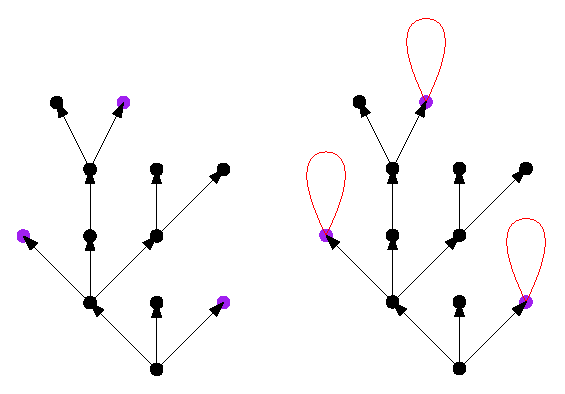
\includegraphics[scale=0.6]{Content/Pictures/black_purple_red_tree.eps}
    \caption{Given a component of $(F^p_n(k),k\geq 1)$ (left), we modify it by sampling independent Bienaymé trees with offspring distributed as $Z^+$ consisting of filler vertices and identifying each dummy leaf with a root of such a tree. The resulting tree (right) is a Bienaymé tree, and the resulting forest $(F^{pr}_n(k),k\geq 1)$ is a Bienaymé forest.}
    \label{fig.blackpurpleredforest}
\end{figure}
The formal procedure is as follows. Suppose we are given $(Y^+(k),S^{+}(k),P_n(k),k\geq 1)$, which encode $(F^p_n(k),k\geq 1)$.
\begin{enumerate}
    \item Let $(Y^{red}(k),k\geq 1)$ be an independent copy of $(Y^+(k),k\geq 1)$, which will encode the pendant subtrees that consist of filler vertices.
    \item Define $\theta_n(k)=k+\min\{j: Y^{red}(j)=-P_n(k-1)\}-P_n(k-1)$. 
    \item Set $\Lambda_n(k)=\max\{j:\theta_n(j)\leq k\}-P_n(\max\{j:\theta_n(j)\leq k\})$. 
    \item We now define \begin{equation}\label{eq.definitionY^{pr}}(Y^{pr}(k),k\geq 1)=(Y^+(\Lambda_n(k))+Y^{red}(k-\Lambda_n(k)),k\geq 1)\end{equation}
    and we let $(F^{pr}(k),k\geq 1)$ be the Bienaymé process encoded by $(Y^{pr}(k),k\geq 1)$, in which $P_n(\max\{j:\theta_n(j)\leq k\})$ of the first $k$ vertices are dummy vertices, $\Lambda_n(k)$ of the first $k$ vertices are true vertices, and the rest are filler vertices. We let $(H^{pr}(k),k\geq 1)$ be the height process corresponding to $(F^{pr}(k),k\geq 1)$.
\end{enumerate}
The subforest consisting of the true vertices and dummy vertices in $F^{pr}(\theta_n(k))$ is, by construction, equal to $F^{p}(k)$. Moreover, $(F^{pr}(k),k\geq 1)$ is a Bienaymé forest. We make the following observations.
\begin{enumerate}
    \item We claim that $$\theta_n(k)=\min\{l: F^p(k)\text{ is a subforest of }F^{pr}(l)\}.$$ Indeed, note that $\min\{j: Y^{red}(j)=-P_n(k-1)\}$ is equal to the number of vertices in the first $P_n(k-1)$ trees in the forest encoded by $Y^{red}$, so that $$\min\{j: Y^{red}(j)=-P_n(k-1)\}-P_n(k-1)$$ is equal to the number of filler vertices we add to $F^p(k)$. Then, $\theta_n(k)$ is the index in $(F^{pr}(k),k\geq 1)$ of the $k^{th}$ black or dummy leaf. 
    \item Note that $\Lambda_n(k)$ is the number of blue vertices amongst the first $k$ vertices. This follows from the fact that $\max\{j:\theta_n(j)\leq k\}$ is the number of blue or dummy leaves amongst the first $k$ vertices. 
    \item By the argument above, $(\Lambda_n(k),k\geq 1)$ only takes steps of size $0$ or $1$. Both $(Y^+(k),k\geq 1)$ and $(Y^{red}(k),k\geq 1)$ are random walks with steps distributed as $Z^+-1$, so, by construction, $(Y^{pr}(k),k\geq 1)$ is a random walk with steps distributed as $Z^+-1$, so $(F^{pr}(k),k\geq 1)$ is a Bienaymé forest with offspring distributed as $Z^+$.
    \item By construction, $(H^{pr}(\theta_n(k)),k\geq 1)$ is the height process corresponding to $(F^p_n(k),k\geq 1)$. Moreover,
   \begin{equation}\label{eq.constructionSp}(S^{+}(k),k\geq 1)=(Y^{pr}(\theta_n(k))-E(\theta_n(k)),k\geq 1),\end{equation}
    where 
    $E(k)$ counts the number of children of the $k^{th}$ vertex in $(F^{pr}(k),k\geq 1)$ that are filler vertices.
\end{enumerate}
Considering the construction above and Corollary \ref{cor.lukasiewiczpathpurplevertices}, in order to prove Proposition \ref{prop.convheightprocesspurple}, it is sufficient to prove the following proposition.
\begin{proposition}\label{prop.heightprocessblackpurplered}
There exists a process $(D_t,t\geq 0)$ such that 
\begin{align*}
    &\left(n^{-1/3}\left[Y^{pr}\left(\theta_n\left(\lfloor n^{2/3}t\rfloor \right)\right)-E\left(\lfloor n^{2/3}t\rfloor \right)\right], n^{-1/3}H^{pr}\left(\theta_n\left(\lfloor n^{2/3}t\rfloor \right)\right),t\geq 0\right)\\
    &\todist\left(\sigma_+D_t,\frac{2}{\sigma_+}\left(D_t-\inf\left\{D_s,s\leq t\right\}\right),t\geq 0\right)
\end{align*}
in $\D(\R_+,\R)^2$ as $n\to \infty$ and $\left(\frac{2}{\sigma_+}\left(D_t-\inf\left\{D_s,s\leq t\right\}\right),t\geq 0\right)$ is the height process corresponding to $(\sigma_+D_t,t\geq 0)$.
\end{proposition} 
We postpone the proof to Appendix \ref{appendix.heightprocessblackpurplered}. 

\subsection{Proof of Theorem \ref{thm.convoutforest}}\label{subsubsec.convaftermeasurechange}
We will now show that the 
We will now combine the convergence of the measure change under rescaling, which is the content of Theorem \ref{thm:measure-change}, and the convergence of the encoding processes of $(F^p(k),k\geq 1)$, which is the content of Proposition \ref{prop.convheightprocesspurple}, in order to prove Theorem \ref{thm.convoutforest}.

\begin{proof}[Proof of Theorem \ref{thm.convoutforest}]
Recall that $\hat{P}_n(k)$ denotes the number of dummy leaves in $\hat{F}_n(k)$. Set $\hat{I}_n(k)=\min\{\hat{S}^{+}_n(l):l\leq k\}$. Then, as shown in Lemma \ref{lemma.sampleoutforest}, the probability that the $(k+1)^{th}$ vertex in $(\hat{F}_n(k),k\geq 1)$ is purple is given by
$$q_{k+1}:=\frac{\hat{S}^-(k)}{\sum_{i=0}^n D^-_i-k-\hat{I}_n(k)}\one_{\left\{\hat{I}_n(k-1)= \hat{I}_n(k)\right\}}.$$
In order to use the results on $(F^p(k),k\geq 1)$, we would like to replace the term $\sum_{i=0}^n D^-_i$ in the denominator by $\mu n$. Therefore, define a new forest $(\hat{F}'_n(k), k\geq 1)$ in which the probability that the $(k+1)^{th}$ vertex is a dummy leaf is
$${q}'_{k+1}:=\frac{\hat{S}^-(k)}{\mu n-k-\hat{I}'_n(k)}\one_{\left\{\hat{I}'_n(k-1)=\hat{I}'_n(k)\right\}},$$
where $\hat{P}'_n(k)$ is the number of dummy leaves in $\hat{F}'_n(k)$, and $\hat{I}'_n(k)$ is the number of components in $\hat{F}'_n(k)$. 
We claim that there exists a coupling such that
$$\sum_{i=1}^{\lfloor n^{2/3}T\rfloor }|q_i-q'_i|\overset{p}{\to}0$$
as $n\to \infty$. 
Indeed, by the convergence in Theorem \ref{theorem.convaftermeasurechange}, 
$$\left(n^{-2/3}\sum_{i=1}^{\lfloor n^{2/3}T\rfloor} \hat{D}^n_i\right)_{n>0}$$ is tight. Moreover, with a slight adaptation to the proof of Lemma \ref{lemma.tightnesssurplusedges}, we can show that $\left(n^{-1/3}\hat{P}'_n\left(\lfloor n^{2/3}T\rfloor \right)\right)_{n>0}$ is tight. This, combined with the convergence under rescaling of $(\hat{Y}^+_n(k),k\geq 1)$, implies that also $\left(n^{-1/3}\hat{I}'_n\left(\lfloor n^{2/3}T\rfloor \right)\right)_{n>0}$ is tight.  Since $D^-_1,\dots,D^-_n$ are i.i.d. random variables with mean $\mu$ and finite variance,
$\left(n^{-1/2}\left(\sum_{i=0}^{n-1}D^-_i-\mu n\right)\right)_{n>0}$ is tight. By using the trivial identity $a/b-c/d=(b(a-c)-c(d-b))/bd$, this implies that
$\left(n^{2/3}\max_{k\leq \lfloor n^{2/3}T\rfloor }|q_k-q'_k|\right)_{n>0}$ is tight, which implies that there exists a coupling such that $\left(\max_{k\leq \lfloor n^{2/3}T\rfloor } |\hat{P}_n(k)-\hat{P}'_n(k)|\right)_{n>1}$ and $\left(\max_{k\leq \lfloor n^{2/3}T\rfloor } |\hat{I}_n(k)-\hat{I}'_n(k)|\right)_{n>1}$ are tight, which implies that, again by $a/b-c/d=(b(a-c)-c(d-b))/bd$, 
$\left(n^{5/6}\max_{k\leq \lfloor n^{2/3}T\rfloor }|q_k-q'_k|\right)_{n>0}$ is tight, which implies that 
$$\sum_{i=0}^{\lfloor n^{2/3}T\rfloor }|q_i-q'_i|\overset{p}{\to}0$$
as $n\to \infty$. 
Therefore, under the right coupling, 
$$\P\left(\max_{k\leq \lfloor n^{2/3} T \rfloor}|\hat{P}_n(k)-\hat{P}'(k)|>0\right)\to 0.$$
In other words, we can couple $(\hat{F}_n(k),k\geq 1)$ and $(\hat{F}'_n(k),k\geq 1)$ in such a way that we do not see the difference on the scale of interest. Therefore, we can show convergence under rescaling of the encoding processes of $(\hat{F}'_n(k),k\geq 1)$ instead. To avoid further complicating notation, we will from now on refer to its encoding processes as $$(\hat{S}^{+}_n(k),\hat{H}_n, \hat{S}^-_n(k), \hat{P}_n(k),k\leq \lfloor n^{2/3}T\rfloor).$$ Then, these processes are constructed out of sample paths of $(\hat{Y}^+(k),\hat{Y}^-(k), k\leq \lfloor n^{2/3}T\rfloor )$ and independent randomness in the exact same way as the sample paths of $$({S}_n^{+}(k),{H}_n^+(k),{S}_n^-(k),P_n(k), k \leq \lfloor n^{2/3}T\rfloor )$$ are constructed out of sample paths of $(Y^+(k),Y^-(k), k\leq \lfloor n^{2/3}T\rfloor )$ and independent randomness. 
We will use the following notation:\begin{align*}
    \hat{S}^{+}_{(n)}&:=\left(n^{-1/3}\hat{S}^{+}_n\left(\lfloor n^{2/3} t \right),0\leq t \leq T\right)\\
    \hat{H}_{(n)}&:=\left(n^{-1/3}\hat{H}_n\left(\lfloor n^{2/3} t \right),0\leq t \leq T\right)\\
    \hat{Y}^+_{(n)}&:=\left(n^{-1/3}\hat{Y}^+\left(\lfloor n^{2/3} t \right),0\leq t \leq T\right)\\
     {S}^{+}_{(n)}&:=\left(n^{-1/3}{S}^{+}_n\left(\lfloor n^{2/3} t \right),0\leq t \leq T\right)\\
    {H}^+_{(n)}&:=\left(n^{-1/3}{H}^+_n\left(\lfloor n^{2/3} t \right),0\leq t \leq T\right)\\
    {Y}^+_{(n)}&:=\left(n^{-1/3}{Y}^+\left(\lfloor n^{2/3} t \right),0\leq t \leq T\right).
\end{align*}
Let $f:D([0,T],\R)^3\to \R$ be a bounded, continuous test-function. Then,
\begin{align*}\E\left[f\left(\hat{Y}^+_{(n)}, \hat{S}^+_{(n)},  \hat{H}_{(n)}\right) \right]&= \E\left[ \E\left[\left. f\left(\hat{Y}^+_{(n)},\hat{S}^+_{(n)},  \hat{H}_{(n)}\right)\right|\hat{Y}^+_{(n)}\right]\right]\\&=\E\left[ \Phi(n,\lfloor n^{2/3} T\rfloor)\E\left[\left.f\left(Y^+_{(n)}, S^+_{(n)},  H^+_{(n)}\right)\right| {Y}^+_{(n)}\right]\right]\\&=\E\left[ \Phi(n,\lfloor n^{2/3} T\rfloor)f\left(Y^+_{(n)},S^+_{(n)},  H^+_{(n)}\right)\right],\end{align*}
where we use that $\E\left[\left. f\left(\hat{Y}^+_{(n)},\hat{S}^+_{(n)},  \hat{H}_{(n)}\right)\right|\hat{Y}^+_{(n)}\right]$ is a bounded, adapted function of $\hat{Y}^+_{(n)}$, and that $\Phi(n,\lfloor n^{2/3} t\rfloor)$ is the measure change from ${Y}^+_{(n)}$ to $\hat{Y}^+_{(n)}$. Then, using Theorem \ref{thm:measure-change} and Proposition \ref{prop.convheightprocesspurple}, following the proof of Theorem 4.1 in \cite{conchon--kerjanStableGraphMetric2020} gives us that 
\begin{align*}
    &\E\left[f\left(\hat{Y}^+_{(n)},\hat{S}^+_{(n)},  \hat{H}_{(n)}\right) \right]\\
    &\to \E\left[\Phi(T)f\left(\sigma_+ B_t,\sigma_+ B^+_t,\frac{2}{\sigma_+}R^+_t,0\leq t \leq T\right)\right].
\end{align*}
Since $$(B^+_t,t\geq 0)=\left(B_t-\frac{\nu_-}{2\sigma_+ \mu}t^2,t\geq 0\right),$$
Lemma \ref{lemma.characterizelimitprocess} implies the convergence under rescaling of $(\hat{S}^+_n(k),\hat{H}_n(k),k\geq 0)$. By Proposition \ref{prop.convheightprocesspurple} , $S^{-}_n$ converges in distribution to a deterministic process under scaling, which will not be affected by the measure change. This completes the proof. 
\end{proof}

\subsection{The convergence of the out-forest holds conditionally on the multigraph being simple}
We will now show that the parts of the directed multigraph we observe up until the timescale in which we are interested are with high probability simple. We will then use an argument by Joseph \cite{josephComponentSizesCritical2014} to show that this implies that Theorem \ref{thm.convoutforest} holds conditional on the resulting multigraph being simple. We let $B_n(k)$ be the number of self-loops and edges created parallel to an existing edge in the same direction as that edge, up until discovery of the $k^{th}$ vertex of $(\hat{F}_n(k),k\geq 1)$. Following \cite{conchon--kerjanStableGraphMetric2020}, we call these anomalous edges. 
\begin{proposition}\label{prop.anomalousedges}
Suppose $\beta<1$. Then we have
$$\P\left(B_n(\lfloor n^\beta \rfloor)>0\right)\to 0$$
as $n\to \infty$.
\end{proposition}
\begin{remark}
We adapt the proof of Lemma 7.1 of \cite{josephComponentSizesCritical2014} and of Proposition 5.3 of \cite{conchon--kerjanStableGraphMetric2020} to the directed setting. A significant complication is caused by the conditioning on $$\left\{\sum_{i=1}^n D^-_i=\sum_{i=1}^n D^+_i\right\}.$$ We observe that in both papers, the proof of the aforementioned result is not fully correct, because the authors use the wrong expression for the probability of sampling an anomalous edge. However, the argument below can be adapted to the setting of \cite{josephComponentSizesCritical2014} and \cite{conchon--kerjanStableGraphMetric2020} to yield a correct proof.
\end{remark}
\begin{proof}
Note that we can only show the convergence of the Radon-Nikodym derivative $\Phi(n,m)$ for $m=O(n^{2/3})$, so it is not straightforward to use the measure change to prove results on the time scale $O(n^\beta)$ for $\beta>2/3$. Therefore, for the proof of this lemma, we will use \emph{Poissonization} to sample $(\mathbf{\hat{D}}_{n,1},\dots,\mathbf{\hat{D}}_{R_n,n})$. This technique was also used by Joseph in \cite{josephComponentSizesCritical2014}. Let $R_n$ be as before, and conditional on $R_n$, let $D^{0,+}_1,\dots,D^{0,+}_{n-R_n}$ i.i.d.\ random variables with the law of $D^+$ conditional on $D^-=0$, and set $S_{n-R_n}=\sum_{i=1}^{n-R_n}D^{0,+}_i$. Fix $\epsilon>0$. There is an $L$ such that with probability at least $1-\epsilon$, both $R_n$ and $S_{n-R_n}$ are within an interval of width $Ln^{1/2}$ around their mean. We condition on this event. Suppose $R_n=r$ and $S_{n-R_n}=s$. 
Let
$$\pi^0(dt,k_1,k_2)=r\P(D^-=k_1,D^+=k_2|D^->0)k_1\exp(-k_1 t)dt$$
be a measure on $\R_+\times \N^2$, and let $\Pi^0$ be a Poisson point process with intensity measure $\pi^0$ conditional on $\Pi^0(\R,\N,\N)=r$. Then, the second and third coordinates of the points in $\Pi^0$ ordered by their first coordinates have the same law as $(\mathbf{\hat{D}}_{n,1},\dots,\mathbf{\hat{D}}_{r,n})$ (before conditioning on the event $\{\sum_{i=1}^nD^-_i=\sum_{i=1}^nD^+_i\}$).  
The intensity of this process is not constant in $t$, so we perform a time change. Define
$$\cL_{\mathbf{D}}(x,y)=\E\left[\left.\exp(-xD^--yD^+)\right|D^->0 \right],$$
and set 
$$\psi(t)=\left(1-\cL_{\mathbf{D}}(\cdot,0)\right)^{-1},$$
so that, by a trivial adaptation of Lemma 4.1 of \cite{josephComponentSizesCritical2014}, for 
$$\pi_r(dt,k_1,k_2):=\P(D^-=k_1,D^+=k_2|D^->0)k_1\exp\left(-k_1 \psi(t/r)\right)\psi'(t/r)dt$$
on $(0,r)\times \N^2$, we have that for $t\in (0,r)$, there exists a probability measure $P_t$ on $\N^2$ such that
$$\pi_r(dt,k_1,k_2)=P_t(D^-=k_1,D^+=k_2)dt.$$
Let ${\Pi}_r$ be a Poisson point process with intensity $\pi_r$.  Now, let $\hat{\Pi}_r$ be a random measure, which is a point process with intensity $\pi_r$, conditioned on 
\begin{enumerate}
    \item $N_r:= \hat{\Pi}_r((0,r),\N,\N)=r$, and 
    \item $\Delta_r:=\int_{(0,r)\times \N^2}(k_1-k_2) \hat{\Pi}_r(dt,k_1,k_2)=s$.
\end{enumerate}
Then, the points of $\hat{\Pi}_r$ ordered by time are distributed as $(\mathbf{\hat{D}}_{n,1},\dots,\mathbf{\hat{D}}_{n,r})$ conditional on $\sum_{i=1}^nD^-_i=\sum_{i=1}^nD^+_i$, $R_n=r$ and $S_{n-R_n}=s$. Let $\hat{\pi}^r_t$ be the marginal intensity measure of $\hat{\Pi}^r$ at time $t$, so that there is a probability measure $\hat{P}^r_t$ on $\N^2$  and a measure $\lambda^r_t$ on $\R_+$ such that $$\hat{\pi}^r_t(dt,k_1,k_2)=\lambda^r_t(dt)\times \hat{P}^r_t(D^-=k_1, D^+=k_2).$$
Note that due to the conditioning, $\lambda^r_t(dt)$ might not be equal to $dt$. However, we claim that, also after conditioning, with high probability, we will have seen between $n^\beta$ and $3n^\beta$ jumps at time $2n^{\beta}$. Indeed,
\begin{align}\begin{split}\label{eq.numberofjumpsinrandommeasure}\P\left(\left.\Pi_r\left((0,2n^{\beta}),\N,\N\right)\not\in (n^\beta,3n^\beta)\right|\Delta_n=0, N_n=n\right)&\leq \frac{\P\left(\sum_{i=1}^{n^\beta}E_i>2n^{\beta}\text{ or }\sum_{i=1}^{3n^\beta}E_i<2n^{\beta}\right)}{\P(\Delta_r=s, N_r=r)}\\
&=O(n^{1/2}\exp(-n^\beta)),\end{split}\end{align}
for $(E_1,E_1,\dots)$ i.i.d. exponential random variables with rate $1$, where the order follows from Cramér's Theorem and the local limit theorem; informally, the numerator is the probability of a large-deviations event, while the denominator is not, since $r$ and $s$ are at distance at most $Ln^{1/2}$ from the mean of $\Delta_r$ and $N_r$. \\
We will use this set-up to show that with high probability, we do not sample anomalous edges in the first $n^\beta$ time-steps of the eDFS. We distinguish between the following types of anomalous edges.\\
Self-loops occur when the out-half-edge of a vertex is paired to an in-half-edge of the same vertex.  Let $B^1_n(k)$ be the number of self-loops that are found up to time $k$. For $v$ explored up to time $\lfloor n^\beta\rfloor$, a vertex with in-degree $d^-_v$ and out-degree $d^+_v$, there are $d^-_v d^+_v$ possible combinations of an in-half-edge and an out-half-edge that form a self-loop connected to $v$. Any of these combinations of half-edges is paired with probability bounded above by 
$$\frac{1}{\sum_{i=\lfloor n^\beta \rfloor+1}^n\hat{D}^-_i}.$$
Parallel edges occur when an out-half-edge of a vertex is paired to an in-half-edge of one of its previously explored children. Let $B^2_n(k)$ be the number of parallel edges that are found up to time $k$. For any vertex $v$ with in-degree $d^-_v$, and a parent $p(v)$ with out-degree $d^+_{p(v)}$, there are at most $d^-_v d^+_{p(v)}$ possible combinations of an in-half-edge and an out-half-edge that form a parallel edge from $p(v)$ to $v$. Again, any of these combinations of half-edges is paired with probability bounded above by 
$$\frac{1}{\sum_{i=\lfloor n^\beta \rfloor+1}^n \hat{D}^-_i}.$$
The last type of anomalous edges is a surplus edge with multiplicity greater than 1. Let $B^3_n(k)$ be the number of surplus edges with multiplicity greater than 1 that are found up to time $k$. For a vertex $w$ with out-degree $d^+_w$ and a vertex $v$ with in-degree $d^-_v$, a multiple surplus edge from $w$ to $v$ can only occur if $v$ is discovered before $w$. In that case, there are at most $(d^+_w)^2(d^-_v)^2$ possible pairs of combinations of half-edges, and each of these pairs appears with probability bounded above by
$$\left(\frac{1}{\sum_{i=\lfloor n^\beta \rfloor+1}^n \hat{D}^-_i}\right)^2.$$
Let $p(i)$ denote the index of the parent of the vertex with index $i$. Also, denote $$\cG^n=\sigma\left(\hat{D}^-_1,\hat{D}^+_1,\dots,\hat{D}^-_n,\hat{D}^+_n \right).$$ Then, by the conditional version of Markov's inequality, 

\begin{align*}\P\left(\left.B^1_n(\lfloor n^\beta \rfloor)>0\right| \cG^n \right)&\leq \frac{\sum_{i=1}^{\lfloor n^\beta \rfloor} \hat{D}^-_i\hat{D}^+_i}{\sum_{i=\lfloor n^\beta \rfloor+1}^n \hat{D}^-_i}\wedge 1,\\
\P\left(\left.B^2_n(\lfloor n^\beta \rfloor)>0\right| \cG^n \right)&\leq \frac{\sum_{i=1}^{\lfloor n^\beta \rfloor} \hat{D}^-_i\E\left[\left.\hat{D}^+_{p(i)}\right|\cG^n\right]}{\sum_{i=\lfloor n^\beta \rfloor+1}^n \hat{D}^-_i}\wedge 1,\\
\P\left(\left.B^3_n(\lfloor n^\beta \rfloor)>0\right| \cG^n \right)&\leq \frac{\sum_{i=1}^{\lfloor n^\beta \rfloor}\sum_{j<i} (\hat{D}^+_i)^2 (\hat{D}^-_j)^2 }{\left(\sum_{i=\lfloor n^\beta \rfloor+1}^n \hat{D}^-_i\right)^2 }\wedge 1,\end{align*}
where we note that $p(i)$ is not adapted to $\cG^n$, because ancestral relations in the tree also depend on the surplus edges. However, we observe that by the Cauchy-Schwarz inequality,
\begin{align*}\sum_{i=1}^{\lfloor n^\beta \rfloor} \hat{D}^-_i\E\left[\left.\hat{D}^+_{p(i)}\right|\cG^n\right]&\leq \left(\sum_{i=1}^{\lfloor n^\beta \rfloor} (\hat{D}^-_i)^2\right)^{1/2}\left(\sum_{i=1}^{\lfloor n^\beta \rfloor} \E\left[\left.\hat{D}^+_{p(i)}\right|\cG^n\right]^2\right)^{1/2}\\
&\leq\left(\sum_{i=1}^{\lfloor n^\beta \rfloor} (\hat{D}^-_i)^2\right)^{1/2}\left(\sum_{i=1}^{\lfloor n^\beta \rfloor} (\hat{D}^+_i)^3\right)^{1/2}\end{align*}
where the last inequality follows from the conditional version of Jensen's inequality and the fact that a vertex with out-degree $d^+$ that is discovered before time $n^\beta$ is the parent of at most $d^+$ vertices that are discovered before time $n^\beta$.

We will show that \begin{equation}\label{eq.conditionalprobanamolousedges}\P\left(\left.B^1_n(\lfloor n^\beta \rfloor)+B^2_n(\lfloor n^\beta \rfloor)+B^3_n(\lfloor n^\beta \rfloor)>0\right| \cG^n \right)\overset{p}{\to}0\end{equation} as $n\to\infty$. The proposition will then follow from the bounded convergence theorem. By the observations above, and the fact that $$\sum_{i=\lfloor n^\beta \rfloor+1}^n \hat{D}^-_i=\sum_{i=1}^n D^-_i-\sum_{i=1}^{\lfloor n^\beta \rfloor -1}\hat{D}^-_i,$$ it is sufficient to show that as $n\to \infty$,
\begin{align}
\frac{1}{n}\int_{(0,2n^\beta)\times \N^2}k_1k_2 \hat{\Pi}_r(dt,k_1,k_2)&\overset{p}{\to}0,\label{eq.convergencemomentpointprocess1}\\
\frac{1}{n}\int_{(0,2n^\beta)\times \N^2}k_1 \hat{\Pi}_r(dt,k_1,k_2)&\overset{p}{\to}0,\label{eq.convergencemomentpointprocess2}\\
\frac{1}{n}\int_{(0,2n^\beta)\times \N^2}k_1^2 \hat{\Pi}_r(dt,k_1,k_2)&\overset{p}{\to}0,\label{eq.convergencemomentpointprocess3}\\
\frac{1}{n}\int_{(0,2n^\beta)\times \N^2}k_2^2 \hat{\Pi}_r(dt,k_1,k_2)&\overset{p}{\to}0,\text{ and }\label{eq.convergencemomentpointprocess4}\\
\frac{1}{n}\int_{(0,2n^\beta)\times \N^2}k_2^3 \hat{\Pi}_r(dt,k_1,k_2)&\overset{p}{\to}0.\label{eq.convergencemomentpointprocess5}\end{align}
We will show \ref{eq.convergencemomentpointprocess1}. The proofs of the other convergences are analogous. \\
Note that, by \eqref{eq.numberofjumpsinrandommeasure}, for $\hat{E}^r_t$ the expectation under $\hat{P}^r_t$, it is sufficient if we show that for some $C$,
\begin{equation}\label{eq.expectationtobound}{\hat{E}}^r_t\left[\hat{D}^-\hat{D}^+\right]
% :=\frac{\E\left[\int_{\N^2}k_1k_2\hat{\Pi}_n(dt,k_1,k_2)\right]}{\E\left[\int_{\N^2}\hat{\Pi}_n(dt,k_1,k_2)\right]}
<C\end{equation}
for all $n$ and $t<2n^\beta$. We note that
$${\hat{E}}^r_t\left[\hat{D}^-\hat{D}^+\right]={E}^r_t\left[\left.\hat{D}^-\hat{D}^+\right| \Delta_r=s, N_r=r\right]={E}^r_t\left[\hat{D}^-\hat{D}^+\frac{\P\left[\left. \Delta_n=s, N_r=r \right| \hat{D}^-_t,\hat{D}^+_t\right]}{\P\left[ \Delta_r=s, N_r=r\right]}\right].$$
By the fact that $\Pi_r$ is a point process, we have that for $k_1$, $k_2$ in $\N$, 
$$\P\left[ \Delta_r=s, N_r=r \left| \hat{D}^-_t=k_1,\hat{D}^+_t=k_2\right.\right]=\P\left[ \Delta_r=s+k_2-k_1, N_r=r-1 \right],$$
so that, since $N_r\sim \operatorname{Poisson}(r)$, and since on the event $\{N_r=r-1\}$ (resp. $\{N_r=r\}$),  $\Delta_r-s$ is the sum of $r-1$ (resp. $r$) i.i.d. random variables with finite variance and mean at most $O(r^{-1/2})$, we observe that 
\begin{align*}
    \P\left[ \Delta_r=s, N_r=r \left| \hat{D}^-_t=k_1,\hat{D}^+_t=k_2\right.\right]&=\omega(r^{-1/2})\text{, and}\\
    \P\left[ \Delta_r=s, N_r=r \right]&=O(r^{-1/2})
\end{align*} for any $k_1$, $k_2$. Therefore, there exists a $C'$ such that
$$\frac{\P\left[ \Delta_r=s, N_r=r \left| \hat{D}^-_t=k_1,\hat{D}^+_t=k_2\right.\right]}{\P\left[ \Delta_r=s, N_r=r\right]}<C'$$
for all $k_1$, $k_2$, $t$ and $n$. If we show that for some $C''$ $${E}^r_t\left[\hat{D}^-\hat{D}^+\right]<C''$$ for all $r$ in the interval that we consider and all $t<2n^\beta$,  \eqref{eq.expectationtobound} follows. We note that by definition of $\pi_r(dt,k_1,k_1)$, 
$${E}^r_t\left[\hat{D}^-\hat{D}^+\right]=\frac{\frac{d^3}{dx^2 dy}\cL_{\mathbf{D}}(x,y)|_{(\psi(t/r),0)}}{\frac{d}{dx}\cL_{\mathbf{D}}(x,y)|_{(\psi(t/r),0)}}.$$
Careful analysis of $\cL_{\mathbf{D}}(x,y)$ and $\psi(s)$ implies that this quantity is bounded uniformly for all $r$ in the interval that we consider and all $t\in(0,2n^\beta)$. We refer the reader to the proof of Lemma A.1 in \cite{josephComponentSizesCritical2014} for the details of a similar argument in the undirected setting. Then, \eqref{eq.expectationtobound} follows. \\
By applying the same techniques, \eqref{eq.convergencemomentpointprocess2}, \eqref{eq.convergencemomentpointprocess3}, \eqref{eq.convergencemomentpointprocess4} and  \eqref{eq.convergencemomentpointprocess5} follow as well, which proves the statement.\end{proof}

% Note that we can only show the convergence of the Radon-Nikodym derivative up to time $O(n^{2/3})$, so it is not straightforward to use the measure change to proof results on a time scale $O(n^\beta)$. Therefore, for the proof of this lemma, we will use a different method, that was introduced by Joseph in \cite{josephComponentSizesCritical2014} referred to as \emph{Poissonization}. We note that $(\mathbf{\hat{D}}_{n,1},\dots,\mathbf{\hat{D}}_{n,n})$ (before conditioning on $\sum_{i=1}^nD^-_i=\sum_{i=1}^nD^+_i$) are distributed as the jumps ordered by jump time in a Poisson process $\Pi^0$ with intensity measure $\pi^0$ on $\R_+\times \N^2$ such that $$\pi^0(dt,k_1,k_2)=n\P(D^-=k_1,D^+=k_2)k_1\exp(-k_1 t)dt$$
% conditionally on $\Pi^0(\R,\N,\N)=n$.
% The intensity of this process is not constant in $t$, so we perform a time change. Define
% $$\cL_{\mathbf{D}}(x,y)=\E\left[\exp(-xD^--yD^+)\right],$$
% and set 
% $$\psi(t)=\left(1-\cL(\cdot,0)\right)^{-1},$$
% so that for 
% $$\pi_n(dt,k_1,k_2):=\P(D^-=k_1,D^+=k_2)k_1\exp\left(-k_1 \psi(t/n)\right)\psi'(t/n)dt$$
% on $(0,n)\times \N^2$, we have that for $t\in (0,n)$, there exists a probability measure $P_t$ on $\N^2$ such that
% $$\pi_n(dt,k_1,k_2)=P_t(D^+=k_1,D^+=k_2)dt.$$
% This is a trivial adaptation of Lemma 4.1 of \cite{josephComponentSizesCritical2014}. Let ${\Pi}_n$ be a decorated point process with intensity $\pi_n$. Now, let $\hat{\Pi}_n$ be a random measure, which is a decorated point process with intensity $\pi_n$, conditionally on 
% \begin{enumerate}
%     \item $N_n:=\hat{\Pi}_n((0,n),\N,\N)=n$, and 
%     \item $\Delta_n:=\int_{(0,n)\times \N^2}(k_1-k_2)\hat{\Pi}_n(dt,k_1,k_2)=0$.
% \end{enumerate}
% Then, the points of $\hat{\Pi}_n$ ordered by time are distributed as $(\mathbf{\hat{D}}_{n,1},\dots,\mathbf{\hat{D}}_{n,n})$ conditionally on $\sum_{i=1}^nD^-_i=\sum_{i=1}^nD^+_i$. Let $\hat{\pi}^n_t$ be the marginal density of $\hat{\Pi}^n$ at time $t$, so that there is a probability measure $\hat{P}^n_t$ on $\N^2$  and a measure $\lambda^n_t$ on $\R_+$ such that $$\hat{\pi}^n_t(dt,k_1,k_2)=\lambda^n_t(dt)\times \hat{P}^n_t(D^-=k_1, D^+=k^2).$$
% Note that due to the conditioning, $\lambda^n_t(dt)$ can be unequal to $dt$. However, we claim that, also after conditioning, with high probability, we will have seen between $n^\beta$ and $3n^\beta$ jumps at time $2n^{\beta}$. Indeed,
% \begin{align}\begin{split}\label{eq.numberofjumpsinrandommeasure}\P\left(\left.\Pi_n\left((0,2n^{\beta}),\N,\N\right)\not\in (n^\beta,3n^\beta)\right|\Delta_n=0, N_n=n\right)&\leq \frac{\P\left(\sum_{i=1}^{n^\beta}E_i>2n^{\beta}\text{ or }\sum_{i=1}^{3n^\beta}E_i<2n^{\beta}\right)}{\P(\Delta_n=0, N_n=n)}\\
% &=O(n^{1/2}\exp(-n))\end{split}\end{align}
% for $(E_1,E_1,\dots)$ i.i.d. exponential random variables with rate $1$, where the order follows from Cramér's Theorem and the local limit theorem. \\
% We will use this set-up to show that with high probability, we do not sample anomalous edges in the first $n^\beta$ time-steps of the eDFS. We distinguish between the following types of anomalous edges.\\
% Self-loops occur when the out-half-edge of a vertex is paired to an in-half-edge of the same vertex.  Let $B^1_n(k)$ be the number of self-loops that are found up to time $k$. For $v$ explored up to time $\lfloor n^\beta\rfloor$, a vertex with in-degree $d^-_v$ and out-degree $d^+_v$, there are $d^-_v d^+_v$ possible combinations of an in-half-edge and an out-half-edge that form a self-loop connected to $v$. Any of these combinations of half-edges is paired with probability bounded above by 
% $$\frac{1}{\sum_{i=\lfloor n^\beta \rfloor+1}^n\hat{D}^-_i}.$$
% Parallel edges occur when an out-half-edge of a vertex is paired to an in-half-edge of one of its previously explored children. Let $B^2_n(k)$ be the number of parallel edges that are found up to time $k$. For any vertex $v$ with in-degree $d^-_v$, and a parent $p(v)$ with out-degree $d^+_{p(v)}$, there are at most $d^-_v d^+_{p(v)}$ possible combinations of an in-half-edge and an out-half-edge that form a parallel edge from $p(v)$ to $v$. Again, any of these combinations of half-edges is paired with probability bounded above by 
% $$\frac{1}{\sum_{i=\lfloor n^\beta \rfloor+1}^n \hat{D}^-_i}.$$
% The last type of anomalous edges is a surplus edge with multiplicity greater than 1. Let $B^3_n(k)$ be the number of surplus edges with multiplicity greater than 1 that are found up to time $k$. For a vertex $w$ with out-degree $d^+_w$ and a vertex $v$ with in-degree $d^-_v$, a multiple surplus edge from $w$ to $v$ can only occur if $v$ is discovered before $w$. In that case, there are at most $(d^+_w)^2(d^-_v)^2$ possible pairs of combinations of half-edges, and each of these pairs appears with probability bounded above by
% $$\left(\frac{1}{\sum_{i=\lfloor n^\beta \rfloor+1}^n \hat{D}^-_i}\right)^2.$$
% Let $p(i)$ denote the index of the parent of the vertex with index $i$. Also, denote $$\cG^n=\sigma\left(\hat{D}^-_1,\hat{D}^+_1,\dots,\hat{D}^-_n,\hat{D}^+_n \right).$$ Then, by a conditional version of Markov's inequality, 

% \begin{align*}\P\left(\left.B^1_n(\lfloor n^\beta \rfloor)>0\right| \cG^n \right)&\leq \frac{\sum_{i=1}^{\lfloor n^\beta \rfloor} \hat{D}^-_i\hat{D}^+_i}{\sum_{i=\lfloor n^\beta \rfloor+1}^n \hat{D}^-_i}\wedge 1,\\
% \P\left(\left.B^2_n(\lfloor n^\beta \rfloor)>0\right| \cG^n \right)&\leq \frac{\sum_{i=1}^{\lfloor n^\beta \rfloor} \hat{D}^-_i\E\left[\left.\hat{D}^+_{p(i)}\right|\cG^n\right]}{\sum_{i=\lfloor n^\beta \rfloor+1}^n \hat{D}^-_i}\wedge 1,\\
% \P\left(\left.B^3_n(\lfloor n^\beta \rfloor)>0\right| \cG^n \right)&\leq \frac{\sum_{i=1}^{\lfloor n^\beta \rfloor}\sum_{j<i} (\hat{D}^+_i)^2 (\hat{D}^-_j)^2 }{\left(\sum_{i=\lfloor n^\beta \rfloor+1}^n \hat{D}^-_i\right)^2 }\wedge 1,\end{align*}
% where we note that $p(i)$ is not adapted to $\cG^n$, because ancestral relations in the tree also depend on surplus edges. However, we observe that by the Cauchy-Schwarz inequality,
% \begin{align*}\sum_{i=1}^{\lfloor n^\beta \rfloor} \hat{D}^-_i\E\left[\left.\hat{D}^+_{p(i)}\right|\cG^n\right]&\leq \left(\sum_{i=1}^{\lfloor n^\beta \rfloor} (\hat{D}^-_i)^2\right)^{1/2}\left(\sum_{i=1}^{\lfloor n^\beta \rfloor} \E\left[\left.\hat{D}^+_{p(i)}\right|\cG^n\right]^2\right)^{1/2}\\
% &\leq\left(\sum_{i=1}^{\lfloor n^\beta \rfloor} (\hat{D}^-_i)^2\right)^{1/2}\left(\sum_{i=1}^{\lfloor n^\beta \rfloor} (\hat{D}^+_i)^3\right)^{1/2}\end{align*}
% where the last inequality follows from the conditional Jensen inequality and the fact that a vertex with out-degree $d^+$ that is discovered before time $n^\beta$ is the parent of at most $d^+$ vertices that are discovered before time $n^\beta$.

% We will show that \begin{equation}\label{eq.conditionalprobanamolousedges}\P\left(\left.B^1_n(\lfloor n^\beta \rfloor)+B^2_n(\lfloor n^\beta \rfloor)+B^3_n(\lfloor n^\beta \rfloor)>0\right| \cG^n \right)\overset{p}{\to}0\end{equation} as $n\to\infty$. Then, the proposition follows from the bounded convergence theorem. By the observations above, and the fact that $$\sum_{i=\lfloor n^\beta \rfloor+1}^n \hat{D}^-_i=\sum_{i=1}^n D^-_i-\sum_{i=1}^{\lfloor n^\beta \rfloor -1}\hat{D}^-_i,$$ it is sufficient to show that as $n\to \infty$,
% \begin{align}
% \frac{1}{n}\int_{(0,2n^\beta)\times \N^2}k_1k_2\hat{\Pi}_n(dt,k_1,k_2)&\overset{p}{\to}0,\label{eq.convergencemomentpointprocess1}\\
% \frac{1}{n}\int_{(0,2n^\beta)\times \N^2}k_1\hat{\Pi}_n(dt,k_1,k_2)&\overset{p}{\to}0,\label{eq.convergencemomentpointprocess2}\\
% \frac{1}{n}\int_{(0,2n^\beta)\times \N^2}k_1^2\hat{\Pi}_n(dt,k_1,k_2)&\overset{p}{\to}0,\label{eq.convergencemomentpointprocess3}\\
% \frac{1}{n}\int_{(0,2n^\beta)\times \N^2}k_2^2\hat{\Pi}_n(dt,k_1,k_2)&\overset{p}{\to}0,\text{ and }\label{eq.convergencemomentpointprocess4}\\
% \frac{1}{n}\int_{(0,2n^\beta)\times \N^2}k_2^3\hat{\Pi}_n(dt,k_1,k_2)&\overset{p}{\to}0.\label{eq.convergencemomentpointprocess5}\end{align}
% We will show \ref{eq.convergencemomentpointprocess1}. The proof of the other equations is analogous. \\
% We start with the proof of \ref{eq.convergencemomentpointprocess1}. Note that by \eqref{eq.numberofjumpsinrandommeasure}, for $\hat{E}^n_t$ the expectation under $\hat{P}^n_t$, it is sufficient if we show that for some $C$,
% \begin{equation}\label{eq.expectationtobound}{\hat{E}}^n_t\left[\hat{D}^-_t\hat{D}^+_t\right]
% % :=\frac{\E\left[\int_{\N^2}k_1k_2\hat{\Pi}_n(dt,k_1,k_2)\right]}{\E\left[\int_{\N^2}\hat{\Pi}_n(dt,k_1,k_2)\right]}
% <C\end{equation}
% for all $n$ and $t<2n^\beta$. We note that
% $${\hat{E}}^n_t\left[\hat{D}^-_t\hat{D}^+_t\right]={E}^n_t\left[\hat{D}^-\hat{D}^+| \Delta_n=0, N_n=n\right]={E}^n_t\left[\hat{D}^-\hat{D}^+\frac{\P\left[ \Delta_n=0, N_n=n | \hat{D}^-_t,\hat{D}^+_t\right]}{\P\left[ \Delta_n=0, N_n=n\right]}\right].$$
% By the fact that $\Pi_n$ is a decorated point process, we have that for $k_1$, $k_2$ in $\N$, 
% $$\P\left[\left. \Delta_n=0, N_n=n \right| \hat{D}^-_t=k_1,\hat{D}^+_t=k_2\right]=\P\left[ \Delta_n=k_2-k_1, N_n=n-1 \right],$$
% so that, since $N_n\sim \operatorname{Poisson}(n)$, and since on $N_n=n-1$ (resp. $N_n=n$),  $\Delta_n$ is the sum of $n-1$ (resp. $n$) i.i.d. mean $0$ random variables with finite variance, there exists a $C'$ such that
% $$\frac{\P\left[ \Delta_n=0, N_n=n | \hat{D}^-_t=k_1,\hat{D}^+_t=k_2\right]}{\P\left[ \Delta_n=0, N_n=n\right]}<C'$$
% for all $k_1$, $k_2$, $t$ and $n$. Therefore, if we show that for some $C''$ $${E}^n_t\left[\hat{D}^-\hat{D}^+\right]<C''$$ for all $n$ and $t<2n^\beta$,  \eqref{eq.expectationtobound} follows. We note that by definition of $\pi_n(dt,k_1,k_1)$, 
% $${E}^n_t\left[\hat{D}^-\hat{D}^+\right]=\frac{\frac{d^3}{dx^2 dy}\cL_{\mathbf{D}}(x,y)|_{(\psi(t/n),0)}}{\frac{d}{dx}\cL_{\mathbf{D}}(x,y)|_{(\psi(t/n),0)}}.$$
% By definition of $\cL_{\mathbf{D}}(x,y)$ and $\psi(s)$, we find that 
% \begin{align*}\frac{d^3}{dx^2 dy}\cL_{\mathbf{D}}(x,y)_{(s,0)}&=-\E[(D^-)^2D^+]+o(1),\\
% \frac{d}{dx}\cL_{\mathbf{D}}(x,y)_{(s,0)}&=-\E[D^-]+o(1)\text{, and}\\
% \psi(s)&=\frac{s}{\mu}+o(s)\end{align*}
% as $s\to 0$. We refer the reader to the proof of Lemma A.1 in \cite{josephComponentSizesCritical2014} for the details of a similar argument in the undirected setting. This implies that 
% $${E}^n_t\left[\hat{D}^-\hat{D}^+\right]=\frac{\E[(D^-)^2D^+]}{\E[D^-]}+o(1)$$
% uniformly in all $t\leq 2n^\beta$, and \eqref{eq.expectationtobound} follows. \\
% By applying the same techniques, \eqref{eq.convergencemomentpointprocess2}, \eqref{eq.convergencemomentpointprocess3}, \eqref{eq.convergencemomentpointprocess4} and  \eqref{eq.convergencemomentpointprocess5} follow as well, which proves the statement.



\begin{corollary}
 Theorem \ref{thm.convoutforest} holds conditionally on the resulting multigraph being simple. 
\end{corollary}
\begin{proof}
Let $\rho(n)=\inf\{k\geq 1:B_n(k)>0\}$, and note that the event that the multigraph formed by the configuration model on $n$ vertices is simple is equal to $\{\rho(n)=\infty\}$. Proposition \ref{prop.anomalousedges} shows that we do not observe any anomalous edges far beyond the timescale in which we explore the largest components of the out-forest. This allows us to conclude that all of the results we prove using the exploration up to time $O(n^{2/3})$ are also true conditioned on $\{\rho(n)=\infty\}$. This follows from the proof of Theorem 3.2 in \cite{josephComponentSizesCritical2014}.
\end{proof}
The results that follow are all obtained by studying the exploration up to time $O(n^{2/3})$, so will also be true conditional on the resulting directed multigraph being simple.

